\documentclass[11pt]{article}
\usepackage[utf8]{inputenc}	% Para caracteres en español
\usepackage{amsmath,amsthm,amsfonts,amssymb,amscd}
\usepackage{multirow,booktabs}
\usepackage[table]{xcolor}
\usepackage{fullpage}
\usepackage{lastpage}
\usepackage{enumitem}
\usepackage{fancyhdr}
\usepackage{mathrsfs}
\usepackage{wrapfig}
\usepackage{setspace}
\usepackage{hyperref}
\usepackage{calc}
\usepackage{multicol}
\usepackage{cancel}
\usepackage[retainorgcmds]{IEEEtrantools}
\usepackage[margin=3cm]{geometry}
\usepackage{amsmath}
\newlength{\tabcont}
\setlength{\parindent}{0.0in}
\setlength{\parskip}{0.05in}
\usepackage{empheq}
\usepackage{framed}
\usepackage[most]{tcolorbox}
\usepackage{xcolor}
\colorlet{shadecolor}{orange!15}
\parindent 0in
\parskip 12pt
\geometry{margin=1in, headsep=0.25in}
\theoremstyle{definition}
\usepackage{pdfpages}
\newtheorem{defn}{Definition}
\newtheorem{reg}{Rule}
\newtheorem{exer}{Exercise}
\newtheorem{note}{Note}
\usepackage{fancyhdr}\usepackage{xcolor}\usepackage{amsmath}\usepackage{amssymb}\pagestyle{fancy}\rhead{}
\newtheorem{theorem}{Theorem}[subsection]
\theoremstyle{definition}
\newtheorem{definition}[theorem]{Definiton}
\newtheorem{example}[theorem]{Example}
\newtheorem{corollary}[theorem]{Corollary}
\newtheorem{lemma}[theorem]{Lemma}
\title{Chapter 9 Review Notes}
\begin{document}
\thispagestyle{empty}
{\LARGE \bf MAT 292 Lecture Notes}\\
{\large Hei Shing Cheung}\\
Ordinary Differential Equations, Fall 2025 \hfill MAT292\\
\\
The up-to-date version of this document can be found at \url{https://github.com/HaysonC/skulenotes}\\

\begin{center}
    ``\textit{ODEs are the bread and butter of engineering. }''
\end{center}
\begin{shaded}
    \textbf{Key Concepts:}
    \begin{itemize}
        \item \textbf{Conflicting Definitions. } This course has multiple definitions for key terms, which may vary between different texts and contexts.
        \item \textbf{Practice Derivatives. } Regular practice with derivatives is essential for mastering ODEs.
        \begin{example}
            The following is a good example of good intuition:

            \textit{What is the antiderivative of $f(x) = \frac{\ln x}{x}$?}

            We know that this is of the form $g \cdot g'$where $g(x) = \ln x$ and $g'(x) = \frac{1}{x}$. Thus, by the rule that:

            \begin{equation}
            \frac{1}{2} \frac{d}{dx} [g(x)]^2 = g(x) g'(x)
            \end{equation}
            we can deduce that:
            $$
            \frac{1}{2} \frac{d}{dx} [(\ln x)^2] = \ln x \cdot \frac{1}{x}
            $$
        \end{example}
        \item \textbf{Practice Linear Algebra. } Familiarity with linear algebra concepts is crucial for understanding ODEs.
    \end{itemize}
\end{shaded}
\section{Examples and Review}
\subsection{What is a Differential Equation?}
\begin{definition}[Differential Equation]
     Any relationship between a variable and its derivatives is called a differential equation. 
\end{definition}

\begin{example}[Newton Second Law]
    Newton's second law states that the force acting on an object is equal to the mass of the object multiplied by its acceleration. Mathematically, this can be expressed as:
    $$
    F = m \frac{d^2x}{dt^2}
    $$
    where \( F \) is the force, \( m \) is the mass, and \( \frac{d^2x}{dt^2} \) is the acceleration (the second derivative of position with respect to time). This is a second-order ordinary differential equation.

    If force is constant, this is a simple form of a differential equation, which we simply rearrange and integrate it (twice), which gives, simply:
    $$
    x(t) = \frac{F}{2m} t^2 + C_1 t + C_0
    $$
    where \( C_1 \) and \( C_0 \) are constants determined by initial conditions.
\end{example}

\begin{example}
    Consider the following ODE:
    $$
    x' = f(t)
    $$
    So we have:
    $$
    \frac{dx}{dt} = f(t)
    $$
    Integrating both sides with respect to \( t \) gives:
    $$
    \int_0^t dx = \int_0^t f(t) \, dt
    $$
    So we have:
    $$
    x(t) = \int_0^t f(t) \, dt + C
    $$
    where \( C \) is a constant of integration. In which initial conditions can be used to determine the value of \( C \).  
\end{example}

\begin{example}[Standard Trick: Turning Higher Order into a System]
    Consider Hooke's Law:
    $$
    F = m\ddot{x} = -kx
    $$
    Then, we let:
    $$
    \begin{cases}
        x_1 = x \\
        x_2 = \dot{x} \\
        \dot{x}_1 = x_2 \\
        \dot{x}_2 = -\frac{k}{m} x_1
    \end{cases}
    $$
    This system can be solved using the techniques for first-order ODEs, as a system by its eigenvalues and eigenvectors:
    $$
    \begin{pmatrix}
        \dot{x}_1 \\
        \dot{x}_2
    \end{pmatrix}
    =
    \begin{pmatrix}
        0 & 1 \\
        -\frac{k}{m} & 0
    \end{pmatrix}
    \begin{pmatrix}
        x_1 \\
        x_2
    \end{pmatrix}
    $$
\end{example}

The above idea scales:

\begin{example}
    Take $F(t, x, \dot{x}, \ddot{x}, \ldots, x^{(n)}) = 0$. Then, we can let:
   \begin{equation}
    \begin{cases}
        x_1 = x \\
        x_2 = \dot{x} \\
        x_3 = \ddot{x} \\
        \vdots \\
        x_n = x^{(n)}
    \end{cases}
    $$
    This allows us to rewrite the original equation as a system of first-order equations:
    $$ 
    \begin{bmatrix}
        \dot{x}_1 \\
        \dot{x}_2 \\
        \vdots \\
        \dot{x}_n
    \end{bmatrix}
    =
    A
    \begin{bmatrix}
        x_1 \\
        x_2 \\
        \vdots \\
        x_n
    \end{bmatrix}
\end{equation}

Where we take $A$ to be the appropriate matrix.
\end{example}

\begin{example}[Exponential Growth]
    You should have already know, that:
    $$
    \frac{dx}{dt} = kx
    $$
    is a first-order linear ODE. The solution to this equation is given by:
    $$
    x(t) = Ce^{kt}
    $$
    where \( C \) is a constant determined by initial conditions.

We could understand the eigenproblems associated with systems of ODEs as an extension of the abovewhere we look for solutions of the form:
\begin{equation}
\begin{bmatrix}
x_1(t) \\
x_2(t) \\
\vdots \\
x_n(t)
\end{bmatrix}
=
e^{At}
\begin{bmatrix}
x_1(0) \\
x_2(0) \\
\vdots \\
x_n(0)
\end{bmatrix}
\end{equation}
where \( A \) is the matrix associated with the system of ODEs. $\exp(At)$ is the matrix exponential of \( At \), which can be computed using various methods, including power series or diagonalization.
\end{example}

\begin{example}[Superposition]
    You should also have already known that the solution to:
    $$ \ddot{x} = -x $$
    is given by:
    $$ x(t) = A \cos(t) + B \sin(t) $$
    where \( A \) and \( B \) are constants determined by initial conditions. The solutions $x_1 = A \cos(t)$ and $x_2 = B \sin(t)$ can be combined to form the general solution. Thus, additional conditions must be satisfied to determine the values of \( A \) and \( B \).
\end{example}
You might have observed that:
\begin{theorem}[Number of Initial Conditions]
    You need as many initial conditions as the order of the ODE to uniquely determine a solution.
\end{theorem}

\begin{example}[Newton's Law of Cooling]
    Let $u(t)$ be the temperature of the object at time $t$. Then, according to Newton's Law of Cooling, we have:
    $$
    \frac{du}{dt} = -k(u - T_a)
    $$
    where \( T_a \) is the ambient temperature, and \( k \) is a positive constant (the transmission coefficient). This is a first-order linear ODE that can be solved using the techniques discussed earlier.

    \textbf{Fixed-Point Solution} We denote the trivial case where \( u(0) = T_a \) as the fixed-point solutionwhere the temperature of the object is equal to the ambient temperature at time \( t = 0 \). It is easy to see that \( u' = 0 \) in this case so \( u(t) = T_a \) for all \( t \).

    One way of solving the general solution is:

    \begin{align*}
        \frac{du}{dt} &= -k(u - T_a) \\
        \int \frac{du}{u - T_a} &= -k \int dt \\
        \ln|u - T_a| &= -kt + C \\
        u - T_a &= e^C e^{-kt} \\
        u &= Be^{-kt} + T_a
    \end{align*}

\end{example}

\begin{definition}[Phase Portraits]
    A phase portrait is a graphical representation of the trajectories of a dynamical system in the phase plane. Each point in the phase plane corresponds to a unique state of the system, and the trajectories represent the evolution of the system over time. Phase portraits are useful for visualizing the behavior of systems of ODEs, particularly in understanding stability and equilibrium points.
\end{definition}

\section{Qualitative Analysis of ODEs}
\subsection{Fixed Points}

We first consider the autonomous system:
\begin{equation}
    \frac{dx}{dt} = f(x)
\end{equation}

\begin{definition}[Autonomous System]
    An autonomous system is a system of ordinary differential equations (ODEs) in which the independent variable (usually time) does not explicitly appear in the equations. In other words, the rate of change of the dependent variable(s) depends only on the current state of the system and not on time itself. Autonomous systems can be expressed in the form:
    $$
    \frac{dx}{dt} = f(x)
    $$
    where \( x \) is the state vector and \( f(x) \) is a function that describes how the state changes over time.
\end{definition}

\begin{definition}[Fixed Point]
    A fixed point (or equilibrium point) of a dynamical system is a point in the phase space where the system remains unchanged over time. Mathematically, for a system described by the differential equation \( \frac{dx}{dt} = f(x) \), a fixed point \( x^* \) satisfies:
    $$
    f(x^*) = 0
    $$
    This means that if the system starts at \( x^* \), it will stay at \( x^* \) for all future times.
\end{definition}

\begin{example}
    Consider $x' = \sin(x)$. The fixed points are given by:
    $$
    \sin(x) = 0 \implies x = n\pi, \quad n \in \mathbb{Z}
    $$
    Thus, the fixed points are \( x = 0, \pm \pi, \pm 2\pi, \ldots \)
\end{example}

\subsubsection{Stability of Fixed Points}
\paragraph{Intuition} Consider a simple pendulum parametized by the angle \( \theta \) from the vertical. The fixed points of this system occur when the pendulum is at rest, which happens at \( \theta = 0 \) (hanging straight down) and \( \theta = \pi \) (inverted position). The case where \textbf{\( \theta = 0 \) is stable}, as small perturbations will cause the pendulum to oscillate around this point. In contrast, \textbf{\( \theta = \pi \) is unstable,} as any small perturbation will cause the pendulum to fall away from this position.

\paragraph{What determines stability?} A fixed point \( x^* \) of a dynamical system \( \frac{dx}{dt} = f(x) \) is classified as:

\begin{subequations}
    stable if:
    \begin{equation}
        \frac{df}{dx} \bigg|_{x=x^*} < 0
    \end{equation}
    unstable if:
    \begin{equation}
        \frac{df}{dx} \bigg|_{x=x^*} > 0
    \end{equation}
    semi-stable if:
    \begin{equation}
        \frac{df}{dx} \bigg|_{x=x^*} = 0
    \end{equation}
\end{subequations}

\begin{proof}
    A demonstration of this will be given in the next section on Linear Stability Analysis \ref{def:linear-stability-analysis}.
\end{proof}

\begin{example}
    Consider the system $x' = \sin(x)$. The fixed points are at \( x = n\pi \)where \( n \in \mathbb{Z} \). To determine the stability of these fixed points, we compute the derivative of \( f(x) = \sin(x) \):
    $$
    \frac{df}{dx} = \cos(x)
    $$
    Evaluating this derivative at the fixed points $x = n\pi$ gives:
    $$
    \cos(n\pi) =\begin{cases}
        1 & \text{if } n \text{ is even (unstable)} \\
        -1 & \text{if } n \text{ is odd (stable)}
    \end{cases}
    $$
    Thus, the fixed points at \( x = 0, \pm 2\pi, \pm 4\pi, \ldots \) are unstable, while the fixed points at \( x = \pm \pi, \pm 3\pi, \pm 5\pi, \ldots \) are stable. 
\end{example}

\paragraph{Drawing Fixed Point Diagrams and Phase Portraits} By visualizing the direction of $x$ due to $x' = f(x)$ on a $x$, $f(x)$ plane (fixed points diagram), we can draw a phase portrait. For the phase portrait, we can demonstrate the fixed points as horizontal lines, and draw points of $x$ that converge to or diverge from these fixed points according to the direction of $x'$.

We draw the fixed point diagram with filled circles for stable fixed points and open circles for unstable fixed points. Arrows indicate the direction of flow towards or away from the fixed points.

\begin{figure}[h!]
    \centering
    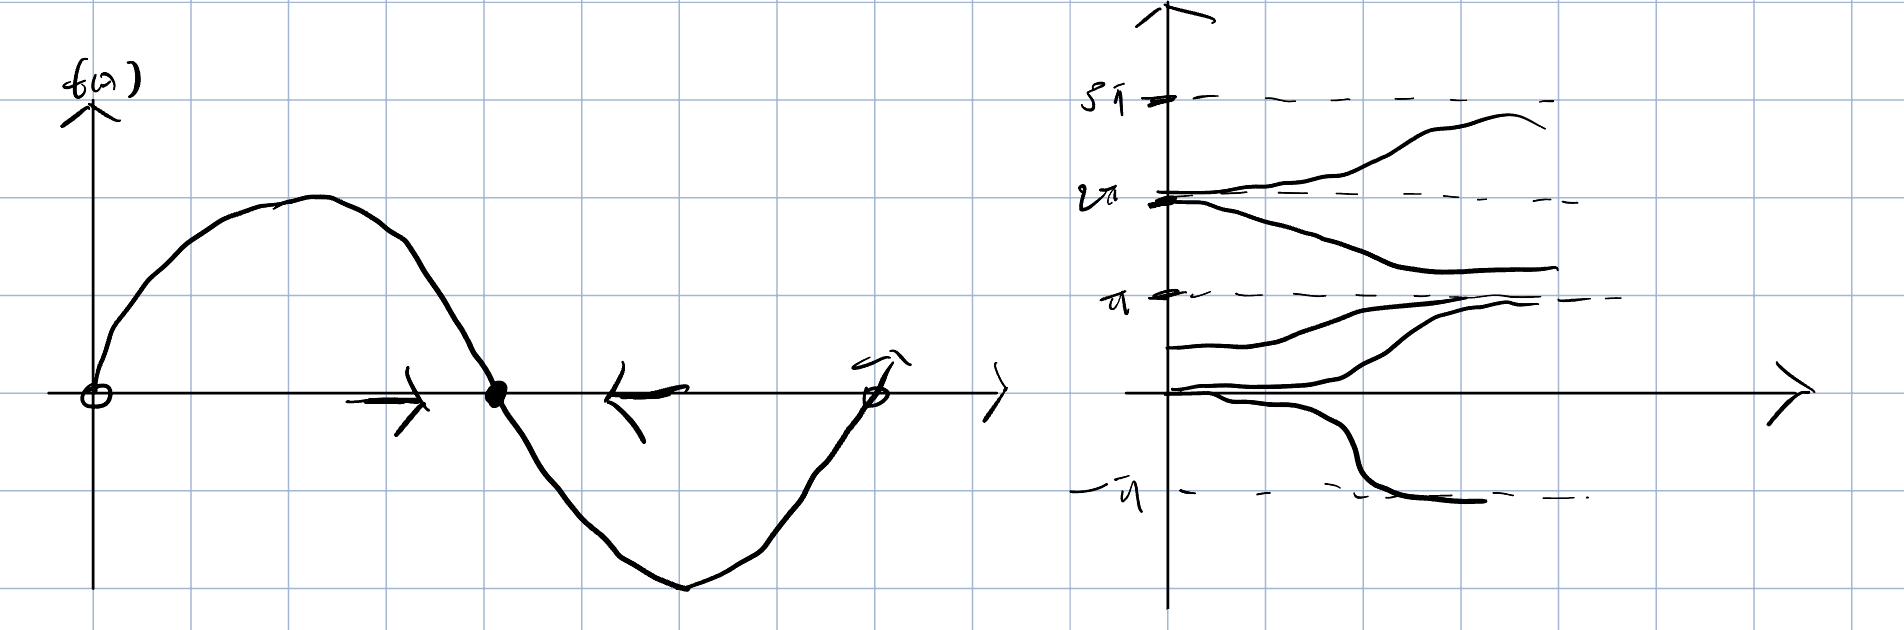
\includegraphics[width=0.6\textwidth]{fixpointdiagram.jpeg}
    \caption{Fixed Point Diagram and Phase Portrait for \( x' = \sin(x) \)}
    \label{fig:fixpointdiagram}
\end{figure}

\begin{theorem}[Non-Intersection of Solutions]
    In a dynamical system described by an ordinary differential equation (ODE) with a unique solution for given initial conditions, the trajectories of different solutions cannot intersect in the phase space. This means that if two solutions start from different initial conditions, they will never cross each other at any point in time.
\end{theorem}
\begin{proof}
    \textbf{Sketch:} If the solutions intersect, then at the point of intersection, the solution is not unique, which contradicts the assumption of uniqueness.
\end{proof}


\paragraph{What Happens When We Consider $t \to -\infty$?} 
\begin{theorem}[Stability Reversal]
    A fixed point that is stable as \( t \to \infty \) becomes unstable as \( t \to -\infty \), and vice versa.
\end{theorem}

\begin{proof}
    This can be understood by considering the time-reversed system. If we denote the time-reversed variable as \( t' = -t \), then the original system \( \frac{dx}{dt} = f(x) \) transforms, by the chain rule, into:
    $$
    \frac{dx}{dt'} = -f(x) 
    $$
    In this new system, the direction of flow is reversed. Therefore, if a fixed point \( x^* \) is stable in the original system (i.e., trajectories approach \( x^* \) as \( t \to \infty \)), it will be unstable in the time-reversed system (i.e., trajectories move away from \( x^* \) as \( t' \to \infty \)). Conversely, an unstable fixed point in the original system becomes stable in the time-reversed system. This demonstrates the reversal of stability when considering \( t \to -\infty \).
\end{proof}
    

\subsubsection{Linear Stability Analysis}

\begin{definition}[Linear Stability Analysis] \label{def:linear-stability-analysis}
    Consider the system $x' = f(x)$. Let $\epsilon$ be any perturbation around a fixed point $x^*$, such that:
    $$x = x^* + \epsilon
    $$
    To analyze the stability of the fixed point, we analyze the behavior of the perturbation $\epsilon(t)$ over time, since $x^*$ is fixed, we have:
    \begin{align*}
        \epsilon' = x' = f(x) &= f(x^* + \epsilon) \\
        \intertext{Ignoring higher order terms in Taylor expansion, we have:}
        &\approx f(x^*) + \epsilon f'(x^*) + \cancel{\frac{1}{2} \epsilon^2 f''(x^*) + \ldots} \\
        &= \epsilon f'(x^*) \quad \text{(since } f(x^*) = 0 \text{)} \\
        \Rightarrow \epsilon' &= f'(x^*) \epsilon
    \end{align*}

    This is a linear ODE in $\epsilon$, which can be solved as:
    $$\epsilon(t) = \epsilon e^{f'(x^*) t}
    $$
    The behavior of $\epsilon(t)z$ depends on the sign of $f'(x^*)$:
    \begin{itemize}
        \item If $f'(x^*) < 0$, then $\epsilon(t) \to 0$ as $t \to \infty$, indicating that the fixed point is stable.
        \item If $f'(x^*) > 0$, then $\epsilon(t) \to \infty$ as $t \to \infty$, indicating that the fixed point is unstable.
        \item If $f'(x^*) = 0$, the linear analysis is inconclusive, and higher-order terms must be considered.
    \end{itemize}
    Thus, the stability of the fixed point can be determined by the sign of $f'(x^*)$.
\end{definition}

\begin{example}
    Consider the system $x' =x^2$. The only fix point is at \( x = 0 \). We have $f'(x) = 2x$, and at the fixed point:
    $$
    f'(0) = 0
    $$
    Thus, the linear stability analysis is inconclusive. We draw the fixed point half filled on the left, and half empty on the right. This is becuase for \( x < 0 \), \( f(x) = x^2 > 0 \), so points to the left of the fixed point move away from it (unstable). For \( x > 0 \), \( f(x) = x^2 > 0 \), so points to the right of the fixed point also move away from it (unstable). Therefore, the fixed point at \( x = 0 \) is unstable.
\end{example}

\subsection{Classification of ODEs}

\begin{shaded}
\paragraph{ODE vs PDE} An ordinary differential equation (ODE) contains functions of a single variable and their derivatives. A partial differential equation (PDE) contains functions of multiple variables and their partial derivatives.
\begin{example}[Heat Equation]
    The heat equation is a PDE that describes how heat diffuses through a given region over time. It is given by:
    $$
    \frac{\partial u}{\partial t} = \alpha \nabla^2 u 
    $$
    where \( u(x, t) \) is the temperature distribution function, \( \alpha \) is the thermal diffusivity constant, and \( \nabla^2 \) is the Laplacian operator.
\end{example}
\begin{example}[Laplace's Equation]
    Laplace's equation is a PDE that describes the behavior of scalar fields such as electric potential and fluid flow. It is given by:
    $$
    \nabla^2 \phi = 0
    $$
    where \( \phi(x, y, z) \) is the scalar potential function, and \( \nabla^2 \) is the Laplacian operator.
    
\end{example}
\end{shaded}
\begin{definition}[Order of an ODE]
    The order of an ordinary differential equation (ODE) is determined by the highest derivative present in the equation.
\end{definition}
\subsubsection{Linearity and Homogeneity of ODEs}
\begin{definition}[Linearity of an ODE]
    An ordinary differential equation (ODE) is considered linear if it can be expressed in the form:
    $$
    a_n(x) \frac{d^n y}{dx^n} + a_{n-1}(x) \frac{d^{n-1} y}{dx^{n-1}} + \ldots + a_1(x) \frac{dy}{dx} + a_0(x) y = g(x)
    $$
    where \( y \) is the dependent variable, \( x \) is the independent variable, \( a_i(x) \) are functions of \( x \), and \( g(x) \) is a known function. In a linear ODE, the dependent variable \( y \) and its derivatives appear to the first power and are not multiplied together. Otherwise, the ODE is considered nonlinear.    
\end{definition}

\begin{definition}[Homogenity of Linear ODEs]
    A linear ordinary differential equation (ODE) is said to be homogeneous if the function \( g(x) \) on the right-hand side of the equation is equal to zero for all values of \( x \). In other words, a homogeneous linear ODE has the form:
    $$
    a_n(x) \frac{d^n y}{dx^n} + a_{n-1}(x) \frac{d^{n-1} y}{dx^{n-1}} + \ldots + a_1(x) \frac{dy}{dx} + a_0(x) y = 0
    $$
    If \( g(x) \) is not identically zero, then the ODE is considered non-homogeneous. Homogeneous linear ODEs have special properties and solution methods that differ from those of non-homogeneous linear ODEs.
\end{definition}

\begin{theorem}[Principle of Superposition]
    Let:
    $$
    a_0(t)y + \dots + a_n(t) \frac{d^n y}{dt^n} =0
    $$
    Assuming that $y_1(t)$ and $y_2(t)$ are two solutions to the above equation, then any linear combination of these solutions $A y_1(t) + B y_2(t)$, where \( A \) and \( B \) are constants, is also a solution.
\end{theorem}
\begin{proof}
    This could be demonstrated by the following derivation:
    \begin{align*}
        & a_0(t)(A y_1 + B y_2) + \dots + a_n(t) \frac{d^n}{dt^n}(A y_1 + B y_2) \\ 
        &= A \left( a_0(t)y_1 + \dots + a_n(t) \frac{d^n y_1}{dt^n} \right) + B \left( a_0(t)y_2 + \dots + a_n(t) \frac{d^n y_2}{dt^n} \right) \\
        &= A \cdot 0 + B \cdot 0 \\
        &= 0
    \end{align*}
    Thus, \( A y_1(t) + B y_2(t) \) is also a solution to the original equation. WLOG, this can be extended to any finite number of solutions.
\end{proof}

Conisder the non-homogeneous case:
\begin{theorem}[General Solution of Non-Homogeneous Linear ODEs]
    Let:
    $$
    a_0(t)y + \dots + a_n(t) \frac{d^n y}{dt^n} =g(t)
    $$
    If \( y_p(t) \) is a particular solution to the non-homogeneous equation, and \( y_h(t) \) is any solution to the corresponding homogeneous equation, then:
    $$
    y(t) = A y_h(t) + y_p(t)
    $$
    is the general solution to the non-homogeneous equation, where \( A \) is an arbitrary constant.
\end{theorem}
\begin{proof}
    \textbf{Sketch:} The solution for the homogeneous part would simply be 0, so the particular solution would be the only solution to the non-homogeneous equation. The general solution is then the sum of the homogeneous and particular solutions.
\end{proof}

\subsubsection{Separable ODEs}
\begin{definition}[Separable ODE]
    An ordinary differential equation (ODE) is said to be separable if it can be expressed in the form:
    $$
    \frac{dy}{dx} = g(x) h(y) = f(x, y)
    $$
    where \( g(x) \) is a function of the independent variable \( x \) only, and \( h(y) \) is a function of the dependent variable \( y \) only. This allows the variables to be separated on opposite sides of the equation, enabling integration with respect to each variable independently:

    \begin{align*}
        \frac{dy}{dx} &= g(x) h(y) \\
        \int \frac{1}{h(y)} dy &= \int g(x) dx \\
        \intertext{Let \( H(y) \) be the antiderivative of \( \frac{1}{h(y)} \) and \( G(x) \) be the antiderivative of \( g(x) \), we have:}
        H(y) &= G(x) + C \\
        \Rightarrow y &= H^{-1}(G(x) + C)
    \end{align*}
    where \( C \) is the constant of integration.
\end{definition}

\paragraph{Remarks} If $g$ and $h$ are continuous, then there need not exist solution in a neighbourhood (open $\epsilon$-ball) of any point $(x_0, y_0)$ so long as $h(y_0) \neq 0$.
\begin{example}[Proof of Uniqueness by Integrating Factor Method]
Consider the IVP
\[
\frac{dx}{dt} = ax, \qquad x(0) = x_0.
\]
Although we know the solution is \( x(t) = x_0 e^{at} \), we will prove that this solution is unique.

Suppose $w(t)$ is any solution of this IVP. Define a change of variables:
$$
y(t) = e^{-at} w(t).
$$
Then, by the product rule,
$$
\frac{dy}{dt} = \frac{d}{dt}\!\left( e^{-at} w(t) \right) 
= -a e^{-at} w(t) + e^{-at} \frac{dw}{dt}.
$$
Since $\tfrac{dw}{dt} = aw(t)$, this becomes
$$
\frac{dy}{dt} = -a e^{-at} w(t) + e^{-at} (a w(t)) = 0.
$$
Thus, $y(t)$ is constant for all $t$. Evaluating at $t=0$ gives
$$
y(0) = e^{-a \cdot 0} w(0) = x_0,
$$
so $y(t) \equiv x_0$. Therefore,
$$
e^{-at} w(t) = x_0 \quad \implies \quad w(t) = x_0 e^{at}.
$$
Hence, the only possible solution of the IVP is
$$
x(t) = x_0 e^{at}.
$$
This shows the solution is unique.
\end{example}

\paragraph{Remark} 
The change of variable 
\[
y(t) = e^{-at} x(t)
\]
allows us to prove the uniqueness of the solution. 
This is essentially the same idea as the integrating factor method.

\begin{example}[Logistic Equation] \label{ex:logistic-equation}
    The logistic equation is a first-order nonlinear separable autonomous ODE that models population growth with a carrying capacity. It is given by:
    $$
    \frac{dx}{dt} = \alpha x \left(1 - x \right)
    $$
    where \( \alpha \) is the growth rate.

    To solve this equation, we can separate the variables:
    \begin{align*}
        \frac{dx}{\alpha x(1 - x)} &= 1 dt \\
        \int \frac{1}{\alpha x(1 - x)} dx &= \int 1 dt \\
        \intertext{Using partial fraction decomposition, we have:}
        \frac{1}{\alpha x(1 - x)} &= \frac{A}{x} + \frac{B}{1 - x} \\
        1 &= A(1 - x) + Bx \\
        1 &= A + (B - A)x \\
        \Rightarrow A &= 1, \quad B - A = 0 \\
        \Rightarrow B &= 1
        \intertext{Thus, we have:}
        \int \left( \frac{1}{\alpha x} + \frac{1}{\alpha (1 - x)} \right) dx &= \int 1 dt \\
        \frac{1}{\alpha} \left( \ln|x| - \ln|1 - x| \right) &= t + C \\
        \ln \left| \frac{x}{1 - x} \right| &= \alpha t + C' \\
        \frac{x}{1 - x} &= e^{\alpha t + C'} = Ce^{\alpha t} \\
        \Rightarrow x(t) &= \frac{Ce^{\alpha t}}{1 + Ce^{\alpha t}}
    \end{align*}

    To analyze the stability of the fixed points, we first find the fixed points by setting \( \frac{dx}{dt} = 0 \):
    $$\alpha x(1 - x) = 0 \implies x = 0 \text{ or } x = 1
    $$
    Next, we compute the derivative of \( f(x) = \alpha x(1 - x) \):
    $$\frac{df}{dx} = \alpha (1 - 2x)
    $$
    Evaluating this derivative at the fixed points, assumeing \( \alpha > 0 \):
    \begin{itemize}
        \item At \( x = 0 \):
        $$\frac{df}{dx} \bigg|_{x=0} = \alpha > 0 \quad \text{(unstable)}
        $$
        \item At \( x = 1 \):
        $$\frac{df}{dx} \bigg|_{x=1} = -\alpha < 0 \quad \text{(stable)}
        $$
    \end{itemize}
    Thus, the fixed point at \( x = 0 \) is unstable, while the fixed point at \( x = 1 \) is stable.
\end{example}
\subsubsection{First-Order Linear ODEs - Integrating Factor Method}
\begin{definition}[First-Order Linear ODE]
    A first-order linear ordinary differential equation (ODE) is an equation of the form:
    \begin{equation}
        \frac{dy}{dx} + P(x)y = Q(x)
    \end{equation}
    where \( P(x) \) and \( Q(x) \) are functions of the independent variable \( x \).
\end{definition}


\begin{definition}[Integrating Factor Method]
    To solve a first-order linear ODE of the form:
    $$
        \frac{dy}{dx} + P(x)y = Q(x)
    $$
    we can use the integrating factor method. The steps are as follows:
    \begin{enumerate}
        \begin{subequations}
    
        \item Compute the integrating factor \( \mu(x) \):
        \begin{equation}
            \mu(x) = \exp\left( \int P(x) \, dx \right)
        \end{equation}
        \begin{shaded}
            This is from the fact that:
        \begin{align*}
            \frac{d\mu}{dx} &= P(x) \mu(x) \quad \text{(by requirement of step \ref{step:integrating-factor-multiplication})} \\
            \Rightarrow \frac{1}{\mu} \frac{d\mu}{dx} &= P(x) \\
            \Rightarrow \int \frac{1}{\mu} \frac{d\mu}{dx} \, dx &= \int P(x) \, dx \\
            \Rightarrow \ln|\mu| &= \int P(x) \, dx \\
            \Rightarrow \mu(x) &= \exp\left( \int P(x) \, dx \right)
        \end{align*}
        \end{shaded}
        \item Multiply both sides of the original ODE by the integrating factor: 
        \begin{equation}
            \mu(x) \frac{dy}{dx} + \mu(x) P(x)y = \mu(x) Q(x)
        \end{equation}
        \item Recognize that the left-hand side is the derivative of \( \mu(x)y \) \label{step:integrating-factor-multiplication}:
        \begin{equation}
            \frac{d}{dx}[\mu(x)y] = \mu(x) Q(x)
        \end{equation}
        \item Integrate both sides with respect to \( x \):
        \begin{equation}
            \mu(x)y = \int \mu(x) Q(x) \, dx + C
        \end{equation}
        where \( C \) is the constant of integration.
        \item Finally, solve for \( y(x) \):
        \begin{equation}
            y(x) = \frac{1}{\mu(x)}\left( \int \mu(x) Q(x) \, dx + C \right)
        \end{equation}
        \end{subequations}
    \end{enumerate}
\end{definition}

\begin{example}
    Consider the IVP involving a first-order linear ODE:
    $$
    y' + \frac{2}{t} y = \frac{\sin t}{t^2}, \quad y(\pi) = 1
    $$

    To solve this IVP using the integrating factor method, we first identify \( P(t) = \frac{2}{t} \) and \( Q(t) = \frac{\sin t}{t^2} \).

    Next, we compute the integrating factor:
    \begin{align*}
        \mu(t) &= \exp\left( \int \frac{2}{t} \, dt \right) \\
        &= \exp\left( 2 \ln |t| \right) \\
        &= |t|^2 = t^2
    \end{align*}

    Multiplying both sides of the original ODE by the integrating factor:
    $$
        t^2 y' + 2ty = \sin t
    $$

    Recognizing the left-hand side as the derivative of \( |t|^2 y \):
    \begin{align*}
        \frac{d}{dt}[t^2 y] &= \sin t \\
        t^2 y &= -\cos t + C \\
        y &= \frac{-\cos t + C}{t^2}
    \end{align*}

    To determine the constant \( C \), we use the initial condition \( y(\pi) = 1 \):
    \begin{align*}
        1 &= \frac{-\cos(\pi) + C}{\pi^2} \\
        \Rightarrow C &= \pi^2 - 1
    \end{align*}

    Thus, the solution to the IVP is:
    \begin{align*}
        y(t) &= \frac{-\cos t + \pi^2 - 1}{t^2}
    \end{align*}
\end{example}

\subsubsection{Exact ODEs}
\begin{definition}[Exact ODE]
    An ordinary differential equation (ODE) of the form:
    \begin{subequations}
    \begin{equation}
        M(x, y) + N(x, y) \frac{dy}{dx} = 0 \quad \text{or equivalently} \quad M(x, y) dx + N(x, y) dy = 0
    \end{equation}
    is said to be exact iff there exists a function \( \psi(x, y) \) such that:
    \begin{equation}
        M_y = \frac{\partial M}{\partial y} = N_x = \frac{\partial N}{\partial x}
    \end{equation}

    This implies a potential function \( \psi(x, y) \) exists such that:
    \begin{equation}
        M_y = \psi_{xy} = \psi_{yx} = N_x
    \end{equation}
    The general solution to the exact ODE is given by:
    \begin{equation}
        d\psi(x, y) = 0 \implies \psi(x, y) = C \quad (\text{By chain rule of $\psi$})
    \end{equation}
    \end{subequations}
    In this case, we can solve the ODE by finding the potential function \( \psi(x, y) \):
    \begin{equation}
        \psi(x, y) = \int M(x, y) \, dx + g(y)
    \end{equation}
    to find \( g(y) \), we can use the fact that:
    \begin{equation}
        \frac{\partial \psi}{\partial y} = \frac{\partial}{\partial y} \left( \int M(x, y) \, dx \right) = \int M_y \, dx = \int N_x \, dx = N(x, y)
    \end{equation}
    We can also solve this from the other direction. Or verify your answer this way.
\end{definition}

\begin{example}
    Consider the exact ODE:
    $$
    (3x^2y^2 + x + \cos{y}) \frac{dy}{dx} = -(2xy^3 + y)
    $$
    We identify \( N(x, y) = 3x^2y^2 + x + \cos{y} \) and \( M(x, y) = 2xy^3 + y \). So \( M_y = N_x = 6x^2y + 1 \), thus the ODE is exact. Then we compute the potential function:
    \begin{align*}
        \psi(x, y) &= \int M(x, y) \, dx \\
        &= \int (2xy^3 + y) \, dx \\
        &= x^2 y^3 + xy + g(y)
        \intertext{To find \( g(y) \), we compute:}
        \frac{\partial \psi}{\partial y} &= 3x^2 y^2 + x + g'(y) \\
        &= N(x, y) = 3x^2 y^2 + x + \cos{y} \\
        \Rightarrow g'(y) &= \cos{y} \\
        \Rightarrow g(y) &= \sin{y}
        \intertext{Thus, the potential function is:}
        \psi(x, y) &= x^2 y^3 + xy + \sin{y}
        \intertext{The general solution to the ODE is then:}
        \psi(x, y) &= C \\
        \Rightarrow x^2 y^3 + xy + \sin{y} &= C
    \end{align*}

    We can verify our answer by computing from the other direction:
    \begin{align*}
        \psi(x, y) &= \int N(x, y) \, dy \\
        &= \int (3x^2 y^2 + x + \cos{y}) \, dy \\
        &= x^2 y^3 + xy + \sin{y} + h(x)
        \intertext{To find \( h(x) \), we compute:}
        \frac{\partial \psi}{\partial x} &= 2x y^3 + y + h'(x) \\
        &= M(x, y) = 2xy^3 + y \\
        \Rightarrow h'(x) &= 0 \\
        \Rightarrow h(x) &= C'
        \intertext{Thus, we obtain the same potential function:}
        \psi(x, y) &= x^2 y^3 + xy + \sin{y} + C'
    \end{align*}
\end{example}

\subsection{Bifurcations}
\begin{definition}[Bifurcation]
    A bifurcation in a dynamical system occurs when a small change in the system's parameters causes a sudden qualitative change in its behavior.

    This can lead to the emergence or disappearance of fixed points, changes in stability, or the onset of periodic or chaotic behavior.
\end{definition}

\begin{definition}[Bifurcation Point]
    A bifurcation point is a specific value of a parameter in a dynamical system at which the qualitative behavior of the system changes. At this point, the system may undergo a bifurcation, leading to changes in the number or stability of fixed points, periodic orbits, or other dynamical features.
    
\end{definition}

\paragraph{Types of Bifurcations} There are several common types of bifurcations in dynamical systems, including:
    \begin{itemize}
        \item Saddle-Node Bifurcation: Two fixed points (one stable and one unstable) collide and annihilate each other as a parameter is varied.
        \item Transcritical Bifurcation: Two fixed points exchange their stability as a parameter is varied.
        \item Pitchfork Bifurcation: A single fixed point splits into three fixed points (one stable and two unstable, or vice versa) as a parameter is varied.
        \item Hopf Bifurcation: A fixed point loses stability and a small amplitude limit cycle (periodic orbit) emerges as a parameter is varied.
    \end{itemize}

\begin{example}
    Consider the ODE:
    $$
    x' = ax(1 - x)
    $$
    This is a classic example of a bifurcation scenario, where the behavior of the system changes qualitatively as the parameter \(a\) is varied. Consider the fix points of the system:
    $$
    x^* = 0, \quad x^* = 1
    $$
    So, we have:
    \begin{itemize}
        \item For \( a < 0 \):
        \begin{itemize}
            \item \( x^* = 0 \) is stable (since \( f'(0) = a < 0 \))
            \item \( x^* = 1 \) is unstable (since \( f'(1) = -a > 0 \))
        \end{itemize}
        \item For \( a > 0 \):
        \begin{itemize}
            \item \( x^* = 0 \) is unstable (since \( f'(0) = a > 0 \))
            \item \( x^* = 1 \) is stable (since \( f'(1) = -a < 0 \))
        \end{itemize}
        \item For \( a = 0 \):
        \begin{itemize}
            \item Both \( x^* = 0 \) and \( x^* = 1 \) are semi-stable (since \( f'(0) = 0 \) and \( f'(1) = 0 \))
        \end{itemize}
        This indicates a bifurcation at \( a = 0 \), where the stability of the fixed points changes.
    \end{itemize}
\end{example}


\begin{example}[Saddle-Node Bifurcation] \label{ex:bifurcation-saddle-node}
    Consider the ODE:
    $$
    x' = x^2 + a
    $$
    This equation has a family of fixed points given by:
    $$
    x^* = \pm\sqrt{-a}
    $$
    For \( a < 0 \), we have two real fixed points, while for \( a > 0 \), there are no real fixed points. At \( a = 0 \), the fixed points collide and disappear, indicating a bifurcation point at \( a = 0 \).
\end{example}

\begin{definition}[Bifurcation Diagram]
    A bifurcation diagram is a visual representation that illustrates how the fixed points of a dynamical system change as a parameter is varied.

    It is a plot of the fixed points against the parameter, showing regions of stability and instability, and we denote stable fixed points with solid lines and unstable fixed points with dashed lines. A bifurcation diagram of Example \ref{ex:bifurcation-saddle-node} is shown below:
    \begin{figure}[h!]
        \centering
        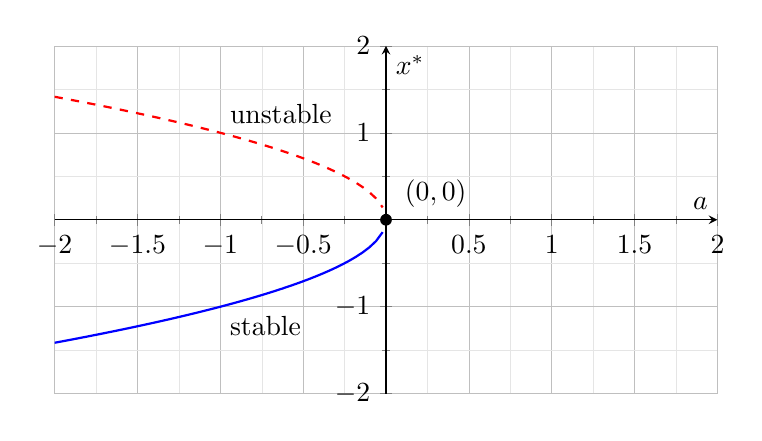
\begin{tikzpicture}
            \begin{axis}[
                axis lines = middle,
                xlabel = \( a \),
                ylabel = \( x^* \),
                ymin = -2, ymax = 2,
                xmin = -2, xmax = 2,
                domain=-2:2,
                samples=100,
                width=10cm,
                height=6cm,
                grid=both,
                minor tick num=1,
                major grid style={line width=.2pt,draw=gray!50},
                minor grid style={line width=.1pt,draw=gray!20},
            ]
            % Stable fixed points
            \addplot[blue, thick] {-sqrt(-x)}; % Stable branch
            \addplot[red, dashed, thick] {sqrt(-x)}; % Stable branch
            
            % Bifurcation point
            \node at (axis cs:0,0) [circle,fill,inner sep=1.5pt]{};
            \node at (axis cs:0.3,0.3) {\( (0,0) \)};

            % Labels
            \node at (axis cs:-1,1) [anchor=south west] {unstable};
            \node at (axis cs:-1,-1) [anchor=north west] {stable};
            \end{axis}
        \end{tikzpicture}
        \caption{Bifurcation Diagram for \( x' = x^2 + a \)}
        \label{fig:bifurcation-diagram}
    \end{figure}

\end{definition}

\begin{example}[Pitchfork Bifurcation]
    Consider the ODE:
    $$
    x' = ax - x^3
    $$
    This equation has a family of fixed points given by:
    $$
    x^* = 0, \quad x^* = \pm\sqrt{a}
    $$
    For \( a \le 0 \), there is one real fixed point at \( x^* = 0 \). For \( a > 0 \), there are three real fixed points: \( x^* = 0 \) (unstable) and \( x^* = \pm\sqrt{a} \) (stable). At \( a = 0 \), the fixed point at \( x^* = 0 \) changes stability, indicating a bifurcation point at \( a = 0 \).

    We can plot the bifurcation diagram for this system as follows:

    \begin{figure}[h!]
        \centering
        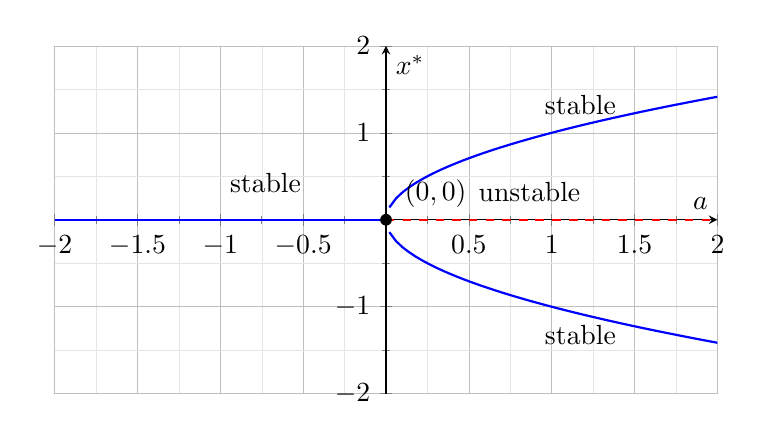
\begin{tikzpicture}
            \begin{axis}[
                axis lines = middle,
                xlabel = \( a \),
                ylabel = \( x^* \),
                ymin = -2, ymax = 2,
                xmin = -2, xmax = 2,
                domain=-2:2,
                samples=100,
                width=10cm,
                height=6cm,
                grid=both,
                minor tick num=1,
                major grid style={line width=.2pt,draw=gray!50},
                minor grid style={line width=.1pt,draw=gray!20},
            ]
            % Stable fixed point for a <= 0
            \addplot[blue, thick, domain=-2:0] {0}; % Stable branch for a <= 0
            % Unstable fixed point for a > 0
            \addplot[red, dashed, thick, domain=0:2] {0}; % Unstable branch for a > 0
            % Stable fixed points for a > 0
            \addplot[blue, thick] {sqrt(x)}; % Stable branch for a > 0
            \addplot[blue, thick] {-sqrt(x)}; % Stable
            % Bifurcation point
            \node at (axis cs:0,0) [circle,fill,inner sep=1.5pt]{};
            \node at (axis cs:0.3,0.3) {\( (0,0) \)};
            % Labels
            \node at (axis cs:-1,0.2) [anchor=south west] {stable};
            \node at (axis cs:0.9,1.1) [anchor=south west] {stable};
            \node at (axis cs:0.9,-1.1) [anchor=north west] {stable};
            \node at (axis cs:0.5,0.1) [anchor=south west] {unstable};
            \end{axis}
        \end{tikzpicture}
        \caption{Bifurcation Diagram for \( x' = ax - x^3 \)}
        \label{fig:pitchfork-bifurcation-diagram}
    \end{figure}
\end{example}

\begin{example}[Transcritical Bifurcation] \label{ex:bifurcation-transcritical}
    Consider the ODE:
    $$
    x' = x(r - x)
    $$
    This equation has a family of fixed points given by:
    $$
    x^* = 0, \quad x^* = r
    $$
    For $r < 0$, \( x^* = 0 \) is stable. For $r > 0$, \( x^* = 0 \) is unstable and \( x^* = r \) is stable. At \( r = 0 \), the stability of the fixed point at \( x^* = 0 \) changes, indicating a bifurcation point at \( r = 0 \). The bifurcation diagram is as follows:
    \begin{figure}[h!]
        \centering
        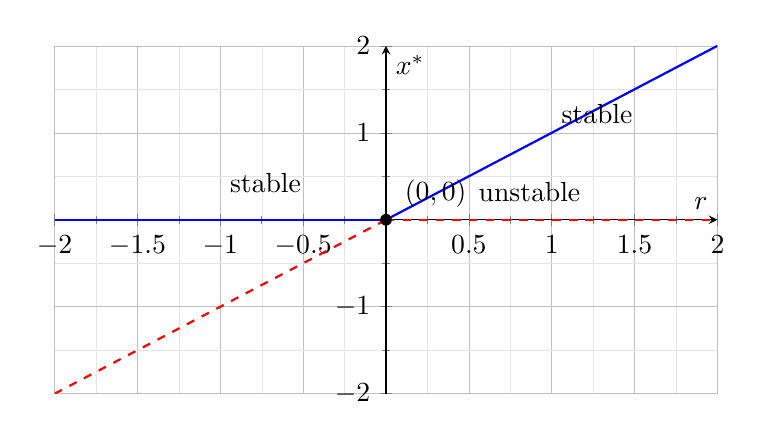
\begin{tikzpicture}
            \begin{axis}[
                axis lines = middle,
                xlabel = \( r \),
                ylabel = \( x^* \),
                ymin = -2, ymax = 2,
                xmin = -2, xmax = 2,
                domain=-2:2,
                samples=100,
                width=10cm,
                height=6cm,
                grid=both,
                minor tick num=1,
                major grid style={line width=.2pt,draw=gray!50},
                minor grid style={line width=.1pt,draw=gray!20},
            ]
            % Stable fixed point for r < 0
            \addplot[blue, thick, domain=-2:0] {0}; % Stable branch for r < 0
            % Unstable fixed point for r < 0
            \addplot[red, dashed, thick, domain=-2:0] {x}; % Unstable branch for r < 0
            % Unstable fixed point for r > 0
            \addplot[red, dashed, thick, domain=0:2] {0}; % Unstable branch for r > 0
            % Stable fixed point for r > 0
            \addplot[blue, thick, domain=0:2] {x}; % Stable branch for r > 0
            % Bifurcation point
            \node at (axis cs:0,0) [circle,fill,inner sep=1.5pt]{};
            \node at (axis cs:0.3,0.3) {\( (0,0) \)};
            % Labels
            \node at (axis cs:-1,0.2) [anchor=south west] {stable};
            \node at (axis cs:1,1) [anchor=south west] {stable};
            \node at (axis cs:0.5,0.1) [anchor=south west] {unstable};
            \end{axis}
        \end{tikzpicture}
        \caption{Bifurcation Diagram for \( x' = x(r - x) \)}
        \label{fig:bifurcation-diagram-2}
    \end{figure}
\end{example}

\paragraph{Linear Stability Analysis and Normal Forms} Consider the ODE in the above example \ref{ex:bifurcation-transcritical}:
We can verify the stability of the fixed points by performing linear stability analysis. Consider $x \sim x^*$ and $r \sim r^*$, such that $|x - x^*| = \epsilon$ and $|r - r^*| = \delta$ for small $\epsilon, \delta > 0$. Then,
\begin{align*}
    f(x, r) &= f(x^*, r^*) + (x-x^*) f_x(x^*, r^*) + (r-r^*) f_r(x^*, r^*) + \\
    &\quad \frac{(x-x^*)^2}{2} f_{xx}(x^*, r^*) + O(\epsilon^3, \delta^2, \epsilon\delta) \\
    &\approx a(x - x^*)^2 + b(r - r^*)
\end{align*}
which we refer to as the normal form of the system. Here, \( a = \frac{1}{2} f_{xx}(x^*, r^*) \) and \( b = f_r(x^*, r^*) \). And that $f_x(x^*, r^*) = 0$ is called a saddle node.


\begin{example}
    Consider the ODE:
    $$
    x' = rx + x^3 - x^5
    $$
    We can find the fixed points by setting \( x' = 0 \), and we have
    $$
    x^\star = 0 \quad \text{or} \quad x^\star = \pm\sqrt{\frac{1 \pm \sqrt{1 + 4r}}{2}}
    $$
    Now, we see the bifurcation points are at \( r = -\frac{1}{4} \) and \( r = 0 \). We have:
    \begin{itemize}
        \item For \( r < -\frac{1}{4} \):
        \begin{itemize}
            \item \( x^* = 0 \) is stable (since \( f'(0) = r < 0 \))
        \end{itemize}
        \item For \( r = -\frac{1}{4} \):
        \begin{itemize}
            \item \( x^* = 0 \) is stable (since \( f'(0) = r < 0 \))
            \item \( x^* = \pm\frac{1}{2} \) are semi-stable (since \( f'(\pm\frac{1}{2}) = 0 \))
        \end{itemize}
        \item For \( -\frac{1}{4} < r < 0 \):
        \begin{itemize}
            \item \( x^* = 0 \) is stable (since \( f'(0) = r < 0 \))
            \item \( x^* = -\sqrt{\frac{1 + \sqrt{1 + 4r}}{2}} \) is stable (since \( f'(-\sqrt{\frac{1 + \sqrt{1 + 4r}}{2}}) < 0 \))
            \item \( x^* = \sqrt{\frac{1 + \sqrt{1 + 4r}}{2}} \) is unstable (since \( f'(\sqrt{\frac{1 + \sqrt{1 + 4r}}{2}}) > 0 \))
        \end{itemize}
        \item For \( r = 0 \):
        \begin{itemize}
            \item \( x^* = 0 \) is semi-stable (since \( f'(0) = 0 \))
            \item \( x^* = -1 \) is stable (since \( f'(-1) < 0 \))
            \item \( x^* = 1 \) is stable (since \( f'(1) < 0 \))
        \end{itemize}
        \item For \( r > 0 \):
        \begin{itemize}
            \item \( x^* = 0 \) is unstable (since \( f'(0) = r > 0 \))
            \item \( x^* = -\sqrt{\frac{1 + \sqrt{1 + 4r}}{2}} \) is stable (since \( f'(-\sqrt{\frac{1 + \sqrt{1 + 4r}}{2}}) < 0 \))
            \item \( x^* = \sqrt{\frac{1 + \sqrt{1 + 4r}}{2}} \) is stable (since \( f'(\sqrt{\frac{1 + \sqrt{1 + 4r}}{2}}) < 0 \))
        \end{itemize}
    \end{itemize}
    The bifurcation diagram is as follows:
    \begin{figure}[h!]
        \centering
        \begin{tikzpicture}
            \begin{axis}[
                axis lines = middle,
                xlabel = {$r$},
                ylabel = {$x^\star$},
                ymin = -2, ymax = 2,
                xmin = -1, xmax = 1,
                samples=200,
                domain=-0.25:1,
                legend style={at={(1.05,1)}, anchor=north west}
            ]
            % Stable and unstable branches from formula
            \addplot[blue, thick, domain=-0.25:1] {
                sqrt((1 + sqrt(1+4*x))/2)
            };
            \addplot[red, dashed, domain=-0.25:1] {
                sqrt((1 - sqrt(1+4*x))/2)
            };
            \addplot[blue, thick, domain=-0.25:1] {
                -sqrt((1 + sqrt(1+4*x))/2)
            };
            \addplot[red, dashed, domain=-0.25:1] {
                -sqrt((1 - sqrt(1+4*x))/2)
            };

            % vertical black dashed line at r = -1/4
            \draw[dashed] (axis cs:-0.25,-2) -- (axis cs:-0.25,2);
            \node at (axis cs:-0.25,2.2) {\( r = -\frac{1}{4} \)};  
            % The trivial equilibrium at x=0
            \addplot[blue, thick, domain=-1:-0.0001] {0}; % stable for r<0
            \addplot[red, dashed, domain=0:1] {0};        % unstable for r>0
            
            % Mark bifurcation points
            \node at (axis cs:-0.25,0.75) [circle,fill,inner sep=1.5pt]{};
            \node at (axis cs:-0.25,-0.75) [circle,fill,inner sep=1.5pt]{};
            \node at (axis cs:0,0) [circle,fill,inner sep=1.5pt]{};
            
            \legend{stable, unstable}
            \end{axis}
        \end{tikzpicture}
        \caption{Bifurcation diagram for $x' = rx + x^3 - x^5$.}
    \end{figure}
\end{example}

\paragraph{Conditions for Bifurcations} Consider $x' = f(x, r)$. Suppose ($x^c, r^c$) is a candidate for a bifurcation point. Then, the following conditions must hold:
\begin{itemize}
    \item \textbf{Equilibrium Condition} $f(x^c, r^c) = 0$ (i.e., $x^c$ is a fixed point for parameter value $r^c$)
    \item \textbf{Non Hyperbolicity Condition} $f_x(x^c, r^c) = 0$ (i.e., the Jacobian at the fixed point has a zero eigenvalue)    
    \item \textbf{Transversality Condition} $f_r(x^c, r^c) \neq 0$ (i.e., the fixed point changes with respect to the parameter)
    \item \textbf{Types of Bifurcations} For different types of bifurcations, we have the following additional conditions:
    \begin{itemize}
        \item \textbf{Saddle-Node Bifurcation} $f_{xx}(x^c, r^c) \neq 0$        
        \item \textbf{Pitchfork Bifurcation} $f_{xx}(x^c, r^c) = 0$ and $f_{xxx}(x^c, r^c) \neq 0$
    \end{itemize}
\end{itemize}
\subsection{Existence and Uniqueness of Solutions}
\begin{example}
    Consider the following IVP:
    $$
    y' = y^{\frac{1}{3}}, \quad y(0) = 0
    $$
    Apart from the trivial solution \( y(t) = 0 \), we can also solve this ODE by separating variables:
    \begin{align*}
        \frac{dy}{y^{1/3}} &= dt \\
        \int y^{-1/3} \, dy &= \int 1 \, dt \\
        \frac{3}{2} y^{2/3} &= t + C \\
        \intertext{Using the initial condition \( y(0) = 0 \), we find \( C = 0 \). Thus, the solution is:}
        y(t) &= \left( \frac{2}{3}(t ) \right)^{3/2}
    \end{align*}
    Thus, we have two solutions to the IVP. Existence is guaranteed, but uniqueness is not.
\end{example}

\begin{example}
    Consider the following IVP:
    $$
    y' = y^2 , \quad y(0) = 1
    $$
    We can solve this ODE by separating variables:
    \begin{align*}
        \frac{dy}{y^2} &= dt \\
        \int y^{-2} \, dy &= \int 1 \, dt \\
        -y^{-1} &= t + C \\
        \intertext{Using the initial condition \( y(0) = 1 \), we find \( C = -1 \). Thus, the solution is:}
        y(t) &= \frac{1}{1 - t}
    \end{align*}
    The solution exists but not globally, as it blows up at \( t = 1 \). Due to the nature of the initial condition, the solution is defined only for \( t < 1 \) to guarantee continuousness.
\end{example}

\begin{theorem}[Existence and Uniqueness Theorem for Linear ODEs]
    Consider the IVP:
    $$
    y' + p(t)y = g(t), \quad y(t_0) = y_0
    $$
    where \( p(t) \) and \( g(t) \) are continuous on an open interval \( I = (\alpha, \beta) \) containing \( t_0 \). Then, there exists a unique solution \( y(t) \) defined on the entire interval \( I \).
\end{theorem}
\begin{proof}
    (\textbf{Existence}) We can use the integrating factor method to find a solution. The integrating factor is given by:
    $$\mu(t) = \exp\left( \int p(t) \, dt \right)
    $$
    Multiplying both sides of the ODE by the integrating factor, we have:
    $$\mu(t) y' + \mu(t) p(t) y = \mu(t) g(t)
    $$
    Integrating both sides with respect to \( t \):
    $$\mu(t)y = \int \mu(s) g(s) \, ds + C
    $$
    We can determine \( C \) using the initial condition \( y(t_0) = y_0 \):
    $$y_0 = \frac{1}{\mu(t_0)}\left( \int_{t_0}^{t_0} \mu(s) g(s) \, ds + y_0 \right)
    $$
    Thus, we have a well defined solution \( y(t) \) defined on the interval \( I \), as long as $p$ and $g$ are continuous on $I$.

    (\textbf{Uniqueness}) Suppose there are two solutions \( y_1(t) \) and \( y_2(t) \) to the IVP, then they must satisfy $y_1(t_0) = y_2(t_0) = y_0$. Define \( z(t) = y_1(t) - y_2(t) \), then \( z(t) \) satisfies:
    $$
    z' + p(t)z = g - g = 0, \quad z(t_0) = y_1(t_0) - y_2(t_0) = 0
    $$
    Apply the same integrating factor method, we have:
    $$\mu(t) z' + \mu(t) p(t) z = 0
    $$
    Integrating both sides with respect to \( t \):
    $$\mu(t)z = \int_{t_0}^{t} 0 \, ds + C = C
    $$
    Using the initial condition \( z(t_0) = 0 \), we find \( C = 0 \). Then, since $\mu$ is a exponential, $\mu > 0$, \( z(t) = 0 \) for all \( t \in I \), which implies \( y_1(t) = y_2(t) \) for all \( t \in I \). Therefore, the solution to the IVP is unique.
\end{proof}

\begin{theorem}[Cauchy-Lipschitz Theorem]
    Consider the IVP:
    $$
    y' = f(t, y), \quad y(t_0) = y_0
    $$
    where \( f(t, y) \) and \( f_y(t, y) \) are continuous on a rectangle \( R = [\alpha, \beta] \times [\gamma, \delta] \). Then, for some point \((t_0, y_0) \in \mathrm{int}(R)\), there exists an interval \( I = (t_0 - h, t_0 + h) \subseteq [\alpha, \beta] \) for some \( 0 < h \le \min(t_0 - \alpha, \beta - t_0) \), such that there exists a unique solution \( y(t) \) defined on the interval \( I \).

\end{theorem}

\begin{proof}
    The proof involves the method of successive approximations (Picard iterations). Which we will not cover here.
\end{proof}

\begin{example}
    To demonstrate that the Cauchy-Lipschitz theorem applies in the linear case, consider the IVP:
    $$
    y' + p(t)y = g(t), \quad y(t_0) = y_0
    $$
    where \( p(t) \) and \( g(t) \) are continuous. We also have \( f_y = -p(t)y + g(t) = -p(t) \). So both \( f \) and \( f_y \) are continuous, thus the Cauchy-Lipschitz theorem guarantees the existence and uniqueness of the solution on some interval around \( t_0 \).
\end{example}

\begin{example}
    Consider the IVP:
    $$
    y' = y^{1/3}, \quad y(0) = 0
    $$
    Here, \( f(t, y) = y^{1/3} \) and \( f_y(t, y) = \frac{1}{3}y^{-2/3} \). The function \( f(t, y) \) is continuous everywhere, but \( f_y(t, y) \) is not continuous at \( y = 0 \). Therefore, the Cauchy-Lipschitz theorem does not apply at the initial condition \( (0, 0) \), which explains why we have multiple solutions to this IVP.
\end{example}

\subsection{Population Dynamics}
\begin{example}[Simple Model]
    Consider the ODE:
    $$
    P' = rP
    $$
    where \( P(t) \) is the population at time \( t \) and \( r \) is the growth rate. This model assumes that the population grows exponentially without any constraints. The solution to this ODE is:
    $$
    P(t) = P_0 e^{rt}
    $$

    \textit{Is this a good model?} Not really, because it assumes unlimited resources and no environmental constraints, which is unrealistic in real-world scenarios.
\end{example}

\begin{example}[A More Realistic Model]
    Consider the logistic growth model:
        $$
        P' = rP\left(1 - \frac{P}{K}\right)
        $$
        where \( K > 0 \) is the carrying capacity of the environment. This model accounts for limited resources and environmental constraints. When $P = K$, the population growth rate becomes zero, indicating that the population has reached its maximum sustainable size.
        The solution to this ODE is:
        $$
        P(t) = \frac{K}{1 + \left(\frac{K - P_0}{P_0}\right)e^{-rt}}
        $$

        This model is more realistic as it predicts that the population will grow rapidly when small, but will slow down and stabilize as it approaches the carrying capacity \( K \).

        \textbf{Note} This is the same ODE considered in Example \ref{ex:logistic-equation}.

        % Two figures side-by-side using minipages, scaled to the column width
        \begin{figure}[h!]
            \centering
            \begin{minipage}[b]{0.48\textwidth}
                \centering
                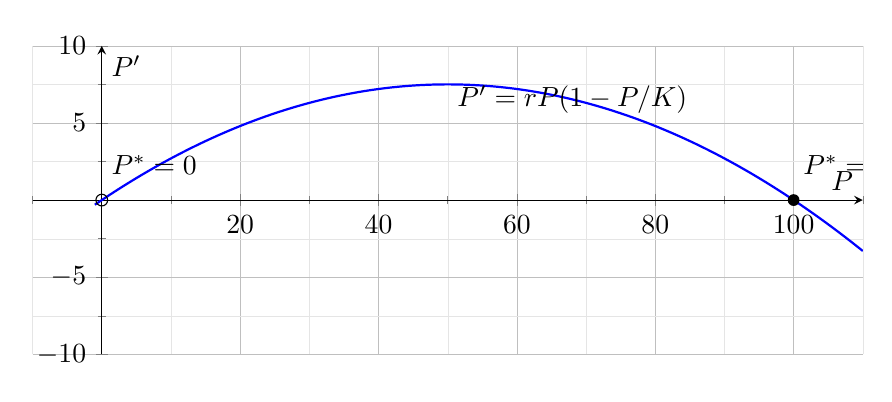
\begin{tikzpicture}
                    \begin{axis}[
                        axis lines = middle,
                        xlabel = \( P \),
                        ylabel = \( P' \),
                        ymin = -10, ymax = 10,
                        xmin = -10, xmax = 110,
                        domain=-1:110,
                        samples=200,
                        width=\linewidth,
                        height=5.5cm,
                        grid=both,
                        minor tick num=1,
                        major grid style={line width=.2pt,draw=gray!50},
                        minor grid style={line width=.1pt,draw=gray!20},
                    ]
                    % Logistic growth curve (example parameters r=0.3, K=100)
                    \addplot[blue, thick] {0.3*x*(1 - x/100)};
                    % Fixed points
                    \node at (axis cs:0,0) [circle, draw, inner sep=1.5pt] {};
                    \node at (axis cs:100,0) [circle,fill,inner sep=1.5pt]{};
                    % Labels
                    \node at (axis cs:50,5) [anchor=south west] {\( P' = rP(1 - P/K) \)};
                    \node at (axis cs:0,1) [anchor=south west] {\( P^* = 0 \)};
                    \node at (axis cs:100,1) [anchor=south west] {\( P^* = K \)};
                    \end{axis}
                \end{tikzpicture}
                \vspace{1mm}

                \small\textbf{(a)} Fixed Point Diagram for the Logistic Growth Model
            \end{minipage}\hfill
            \begin{minipage}[b]{0.48\textwidth}
                \centering
                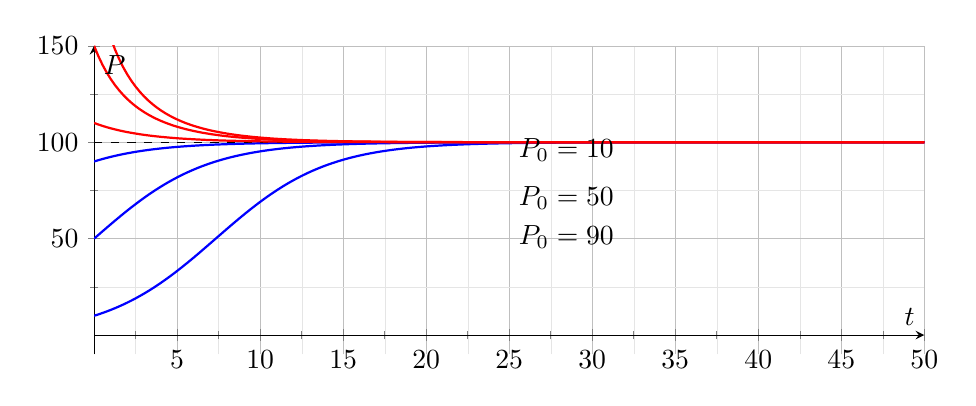
\begin{tikzpicture}
                    \begin{axis}[
                        axis lines = middle,
                        xlabel = \( t \),
                        ylabel = \( P \),
                        ymin = -10, ymax = 150,
                        xmin = 0, xmax = 50,
                        domain=0:50,
                        samples=200,
                        width=\linewidth,
                        height=5.5cm,
                        grid=both,
                        minor tick num=1,
                        major grid style={line width=.2pt,draw=gray!50},
                        minor grid style={line width=.1pt,draw=gray!20},
                    ]
                    % Logistic growth solution curves for different initial conditions (K=100, r=0.3)
                    \addplot[blue, thick] {100/(1 + (100/10 - 1)*exp(-0.3*x))}; % P0 = 10
                    \addplot[blue, thick] {100/(1 + (100/50 - 1)*exp(-0.3*x))}; % P0 = 50
                    \addplot[blue, thick] {100/(1 + (100/90 - 1)*exp(-0.3*x))}; % P0 = 90

                    % carrying capacity line
                    \draw[dashed] (axis cs:0,100) -- (axis cs:50,100);
                    \node at (axis cs:50.5,100) [anchor=west] {\( P = K \)};

                    \addplot[red, thick] {100/(1 + (100/190 - 1)*exp(-0.3*x))}; % P0 = 10
                    \addplot[red, thick] {100/(1 + (100/150- 1)*exp(-0.3*x))}; % P0 = 50
                    \addplot[red, thick] {100/(1 + (100/110 - 1)*exp(-0.3*x))}; % P0 = 90

                    % Labels for initial conditions
                    \node at (axis cs:25,85) [anchor=south west] {\( P_0 = 10 \)};
                    \node at (axis cs:25,60) [anchor=south west] {\( P_0 = 50 \)};
                    \node at (axis cs:25,40) [anchor=south west] {\( P_0 = 90 \)};
                    \end{axis}
                \end{tikzpicture}
                \vspace{1mm}

                \small\textbf{(b)} Sample solution trajectories (different \(P_0\))
            \end{minipage}
            \caption{Logistic growth: (a) fixed-point diagram; (b) sample solution trajectories for different initial conditions.}
            \label{fig:logistic-growth-side-by-side}
        \end{figure}
\end{example}

\begin{example}[Logistics with Threshold]
    Now we introduce a threshold \( T \) below which the population cannot sustain itself:
        $$
        P' = rP\left(1 - \frac{P}{K}\right)\left(\frac{P}{T} - 1\right)
        $$
        This model introduces an Allee effect, where the population growth rate becomes negative when the population is below the threshold \( T \). The fixed points of this system are:
        $$
        P^* = 0, \quad P^* = T, \quad P^* = K
        $$
        The stability of these fixed points can be analyzed as follows:
        \begin{itemize}
            \item \( P^* = 0 \) is stable (since \( f'(0) < 0 \))
            \item \( P^* = T \) is unstable (since \( f'(T) > 0 \))
            \item \( P^* = K \) is stable (since \( f'(K) < 0 \))
        \end{itemize}

    A phase plot and sample solution trajectories are shown below (the sketch shows guides at \(P=T\) and \(P=K\), and sample trajectories that converge to \(K\) or diverge to \(0\)):

        \begin{figure}[h!]
            \centering
            \begin{minipage}[b]{0.48\textwidth}
                \centering
                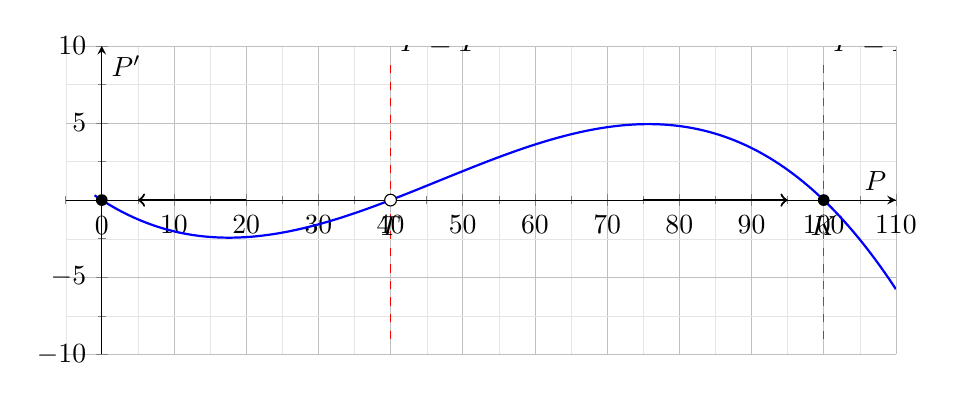
\begin{tikzpicture}
                    \begin{axis}[
                        axis lines = middle,
                        xlabel = \( P \),
                        ylabel = \( P' \),
                        ymin = -10, ymax = 10,
                        xmin = -5, xmax = 110,
                        domain=-1:110,
                        samples=200,
                        width=\linewidth,
                        height=5.5cm,
                        grid=both,
                        minor tick num=1,
                        major grid style={line width=.2pt,draw=gray!50},
                        minor grid style={line width=.1pt,draw=gray!20},
                    ]
                    % Logistic growth with threshold curve (example parameters r=0.3, K=100, T=40)
                    \addplot[blue, thick] {0.3*x*(1 - x/100)*(x/40 - 1)};
                    % Axis baseline and vertical guides at P=T and P=K
                    \addplot[black] coordinates {(0,0) (110,0)}; % P-axis
                    \draw[red,dashed]  (axis cs:40,-9) -- (axis cs:40,9) node[black, above right] {\(P=T\)};
                    \draw[teal,dashed] (axis cs:100,-9) -- (axis cs:100,9) node[black, above right] {\(P=K\)};
                    % Fixed points markers on P-axis (at P'=0)
                    \node at (axis cs:0,0) [circle,fill,inner sep=1.5pt,label=below:{\(0\)}] {};
                    \node at (axis cs:40,0) [circle,draw,fill=white,inner sep=1.5pt,label=below:{\(T\)}] {};
                    \node at (axis cs:100,0) [circle,fill,inner sep=1.5pt,label=below:{\(K\)}] {};
                    % Flow direction arrows on P-axis (qualitative)
                    \draw[->,thick] (axis cs:20,0) -- (axis cs:5,0);    % 0<T: P decreases (left)                    \draw[->,thick] (axis cs:45,0) -- (axis cs:70,0.6);   % T<K: P increases (right)
                    \draw[->,thick] (axis cs:75,0) -- (axis cs:95,0);   % >K: P decreases (left)
                   
                    \end{axis}
                \end{tikzpicture}
                \vspace{1mm}    
                \small\textbf{(a)} Phase diagram (fixed points and flow)
            \end{minipage}\hfill
            \begin{minipage}[b]{0.48\textwidth}
                \centering
                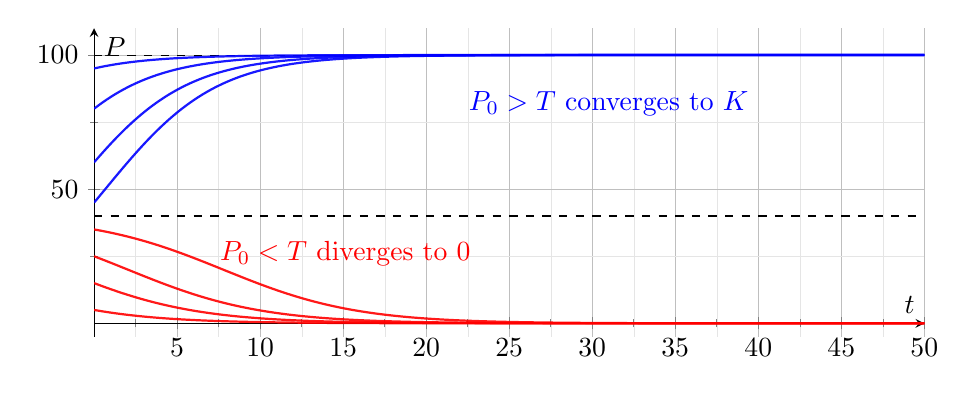
\begin{tikzpicture}
                    \begin{axis}[
                        axis lines = middle,
                        xlabel = \( t \),
                        ylabel = \( P \),
                        ymin = -5, ymax = 110,
                        xmin = 0, xmax = 50,    
                        domain=0:50,
                        samples=200,
                        width=\linewidth,
                        height=5.5cm,
                        grid=both,
                        minor tick num=1,   
                        major grid style={line width=.2pt,draw=gray!50},
                        minor grid style={line width=.1pt,draw=gray!20},
                    ]
                    % carrying capacity line
                    \draw[dashed] (axis cs:0,100) -- (axis cs:50,100);
                    \node at (axis cs:50.5,100) [anchor=west] {\( P = K \)};
                    % threshold line (visual)
                    \draw[dashed] (axis cs:0,40) -- (axis cs:50,40);
                    \node at (axis cs:50.5,40) [anchor=west] {\( P = T \)};
                    % Sample solution trajectories (qualitative sketches)
                    % Below-threshold -> decline to 0 (four examples)
                    \addplot[red, thick, opacity=0.9, domain=0:50, samples=200]
                        {40/(1 + (40/35 - 1)*exp(0.25*x))};
                    \addplot[red, thick, opacity=0.9, domain=0:50, samples=200]
                        {40/(1 + (40/25 - 1)*exp(0.25*x))};
                    \addplot[red, thick, opacity=0.9, domain=0:50, samples=200]
                        {40/(1 + (40/15 - 1)*exp(0.25*x))};
                    \addplot[red, thick, opacity=0.9, domain=0:50, samples=200]
                        {40/(1 + (40/5  - 1)*exp(0.25*x))};
                    \node[red] at (axis cs:7,26) [anchor=west] {\(P_0<T\) diverges to $0$};
                    % Above-threshold -> grow to K (four examples)
                    \addplot[blue, thick, opacity=0.9, domain=0:50, samples=200]
                        {100/(1 + (100/45 - 1)*exp(-0.3*x))};
                    \addplot[blue, thick, opacity=0.9, domain=0:50, samples=200]
                        {100/(1 + (100/60 - 1)*exp(-0.3*x))};
                    \addplot[blue, thick, opacity=0.9, domain=0:50, samples=200]
                        {100/(1 + (100/80 - 1)*exp(-0.3*x))};
                    \addplot[blue, thick, opacity=0.9, domain=0:50, samples=200]
                        {100/(1 + (100/95 - 1)*exp(-0.3*x))};
                    \node[blue] at (axis cs:40,82) [anchor=east] {\(P_0>T\) converges to $K$};
                    \end{axis}
                \end{tikzpicture}
                \vspace{1mm}    
                \small\textbf{(b)} Sample time trajectories: convergence to \(K\) or collapse to \(0\)
            \end{minipage}
            \caption{Logistic growth with threshold: (a) phase portrait with horizontal guides at \(P=T\) and \(P=K\); (b) qualitative solution trajectories showing convergence and divergence relative to the threshold.}
            \label{fig:logistic-growth-threshold-side-by-side}
        \end{figure}
\end{example}

\begin{example}[Harvesting Model]
    Consider a population model with harvesting:
    $$
    P' = rP\left(1 - \frac{P}{K}\right) - H
    $$
    where \( H \) is the constant harvesting rate. The fixed points of this system are given by solving:
    $$
    rP\left(1 - \frac{P}{K}\right) - H = 0
    $$
    This leads to a quadratic equation in \( P \):
    $$
    P^2 - KP + \frac{KH}{r} = 0
    $$
    The solutions to this equation are:
    $$
    P^* = \frac{K \pm \sqrt{K^2 - 4\frac{KH}{r}}}{2}
    $$
    The stability of these fixed points can be analyzed as follows:
    \begin{itemize}
        \item If \( H < \frac{rK}{4} \), there are two real fixed points: one stable and one unstable.
        \item If \( H = \frac{rK}{4} \), there is one real fixed point (a saddle-node bifurcation point).
        \item If \( H > \frac{rK}{4} \), there are no real fixed points, indicating that the population will decline to extinction.
    \end{itemize}
    \textbf{Fixed Point Diagram} A fixed point diagram is shown below:
        \begin{figure}[h!]
            \centering
            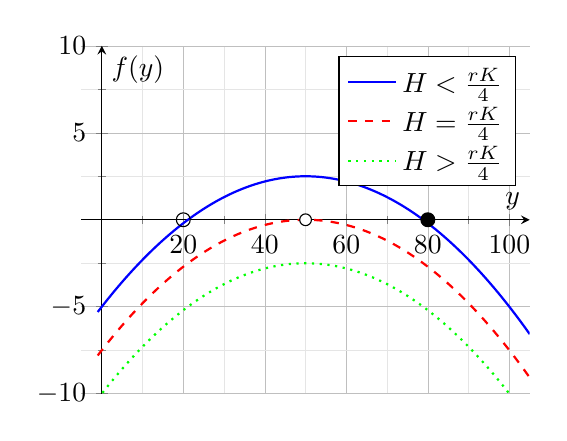
\begin{tikzpicture}
                \begin{axis}[
                    axis lines = middle,
                    xlabel = \( y \),
                    ylabel = \( f(y) \),
                    ymin = -10, ymax = 10,
                    xmin = -5, xmax = 105,
                    domain=-1:105,
                    samples=200,
                    width=0.6\linewidth,
                    height=6cm,
                    grid=both,
                    minor tick num=1,
                    major grid style={line width=.2pt,draw=gray!50},
                    minor grid style={line width=.1pt,draw=gray!20},
                    legend pos=north east,
                ]
                % Quadratic curve for different H values with legend entries
                \addplot[blue, thick] {0.3*x*(1 - x/100) - 5};
                \addlegendentry{\(H < \tfrac{rK}{4}\)}
                \addplot[red, thick, dashed] {0.3*x*(1 - x/100) - 7.5};
                \addlegendentry{\(H = \tfrac{rK}{4}\)}
                \addplot[green, thick, dotted] {0.3*x*(1 - x/100) - 10};
                \addlegendentry{\(H > \tfrac{rK}{4}\)}
                % Fixed points using plot marks (uses built-in plot labeling via legend)
                \addplot[black, only marks, mark=o, mark size=2.5pt] coordinates {(20,0)};
                \addplot[black, only marks, mark=*, mark size=2.5pt] coordinates {(80,0)};
                % semi-filled marker for intermediate / degenerate fixed point
                % half-filled marker: right half black, left half white
                \node at (axis cs:50,0) [circle, draw, fill=white, inner sep=1.5pt] {};
                \end{axis}
            \end{tikzpicture}
            \caption{Fixed point diagram for the harvesting model with different harvesting rates \(H\).}
        \end{figure}

     \textbf{Bifurcation Diagram} This is a classic example of a saddle-node bifurcation (0 to 2 fixed points). The bifurcation point is at $(k/2, 4h/K)$. The bifurcation diagram is shown below:
        \begin{figure}[h!]
            \centering
            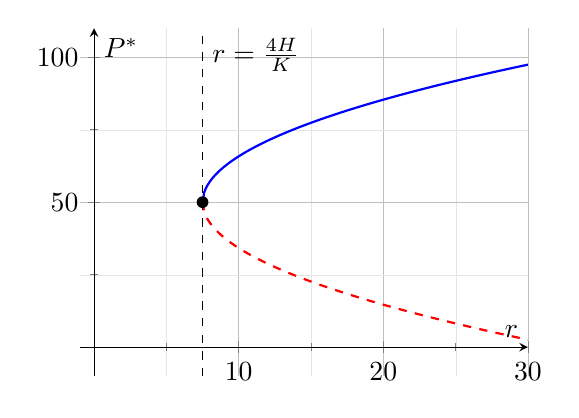
\begin{tikzpicture}
                \begin{axis}[
                    axis lines = middle,
                    xlabel = \( r \),
                    ylabel = \( P^* \),
                    ymin = -10, ymax = 110,
                    xmin = -1, xmax = 30,
                    domain=0:30,
                    samples=200,
                    width=0.6\linewidth,
                    height=6cm,
                    grid=both,
                    minor tick num=1,
                    major grid style={line width=.2pt,draw=gray!50},
                    minor grid style={line width=.1pt,draw=gray!20},
                ]
                % Bifurcation curve (example parameters r=0.3, K=100)
                \addplot[blue, thick, domain=7.5:30] {50 + 10*sqrt(x-7.5)};
                \addplot[red, thick, dashed, domain=7.5:30] {50 - 10*sqrt(x-7.5)};
                \draw[dashed] (axis cs:7.5,-10) -- (axis cs:7.5,110);
                \node at (axis cs:7.5,110) [anchor=north west] {\( r = \frac{4H}{K} \)};
                % Mark bifurcation point
                \node at (axis cs:7.5,50) [circle,fill,inner sep=1.5pt]{};
                \end{axis}
            \end{tikzpicture}
            \caption{Bifurcation diagram for the harvesting model showing the saddle-node bifurcation at \(H = \frac{rK}{4} \).}
        \end{figure}

\end{example}

\begin{theorem}[ID Autonomous ODEs are Monotonic]
    Consider the ODE:
    $$
    y' = f(y)
    $$
    where \( f(y) \) is continuous. Then, the solution \( y(t) \) is monotonic on its interval of existence.
    
\end{theorem}
\begin{proof}
    WLOG, suppose \( f(y_0) > 0 \). For the sake of contradiction, suppose \( y(t) \) is not monotonic. Then, there exists \( t_1 > t_0 \) such that \( y(t_1) < y(t_0) \). By the Intermediate Value Theorem, there exists \( t_2 \in (t_0, t_1) \) such that \( y(t_2) = y(t_0) \). By the Mean Value Theorem, there exists \( c \in (t_0, t_2) \) such that:
    $$\frac{y(t_2) - y(t_0)}{t_2 - t_0} = y'(c)$$
    But \( y(t_2) = y(t_0) \), so the left-hand side is zero. Thus, \( y'(c) = 0 \). However, since \( f(y) \) is continuous and \( f(y_0) > 0 \), there exists a neighborhood around \( y_0 \) where \( f(y) > 0 \). This contradicts the assumption that \( y'(c) = 0 \). Therefore, \( y(t) \) must be monotonic.
\end{proof}

\begin{definition}[System of ODEs]
    A system of ODEs is a set of coupled first-order ODEs of the form:
    $$
    \begin{cases}
    x_1' = f_1(t, x_1, x_2, \ldots, x_n) \\
    x_2' = f_2(t, x_1, x_2, \ldots, x_n) \\
    \vdots \\
    x_n' = f_n(t, x_1, x_2, \ldots, x_n)
    \end{cases}
    $$
    where \( x_i(t) \) are the state variables and \( f_i(t, x_1, x_2, \ldots, x_n) \) are given functions.
\end{definition}
\subsection{Systems of ODEs}

\begin{definition}[Two-Species Interaction Model]
    Consider a model of two species interacting, such as predator-prey dynamics:
    $$
    \begin{cases}
    x' = x(r_1 - ax -by) \\
    y' = y(r_2 + cx - dy)
    \end{cases}
    $$
    where \( x(t) \) and \( y(t) \) are the populations of the two species, \( r_1, r_2, a, b, c, d \) are constants representing:
    \begin{itemize}
        \item \( r_1, r_2 \): intrinsic growth rates of species \( x \) and \( y \)
        \item \( a, d \): intrinsic carrying capacity coefficients
        \item \( b, c \): interspecific coefficients representing the effect of one species on the other
    \end{itemize}
\end{definition}

\begin{example}[Lotka-Volterra Model]
    Now, consider the classic Lotka-Volterra predator-prey model:
    $$
    \begin{cases}
    x' &= ax - bxy \\
    y' &= -cy + dxy \\
    (x(0), y(0)) &= (x_0, y_0)
    \end{cases}
    $$
    where \( x(t) \) is the prey population, \( y(t) \) is the predator population, and \( a, b, c, d \) are positive constants representing:
    \begin{itemize}
        \item \( a \): growth rate of prey in the absence of predators
        \item \( b \): predator efficiency (how many prey are eaten per predator per unit time)
        \item \( c \): natural death rate of predators in the absence of prey
        \item \( d \): conversion efficiency (how many predators are born per prey eaten)
    \end{itemize}
    Consider the fixed points of this system by setting \( x' = 0 \) and \( y' = 0 \). Then we have:
    $$
    (x^*, y^*) = (0, 0) \quad \text{and} \quad (x^*, y^*) = \left(\frac{c}{d}, \frac{a}{b}\right)
    $$
    The case where \( (x^*, y^*) = (0, 0) \) is trivial (extinction of both species). The non-trivial fixed point \( \left(\frac{c}{d}, \frac{a}{b}\right) \) represents a coexistence equilibrium where the rate of the prey being eaten is the rate of the prey being born.
\end{example}

We can further analyze this by considering Nullclines.

\begin{definition}[Nullclines]
    Nullclines are curves in the phase plane where the derivative of \textbf{one of the variables} is zero. For the Lotka-Volterra model, the nullclines are given by:
    \begin{itemize}
        \item Prey nullcline (\( x' = 0 \)): \( y = \frac{a}{b} \) (horizontal line)
        \item Predator nullcline (\( y' = 0 \)): \( x = \frac{c}{d} \) (vertical line)
    \end{itemize}
    The intersection of these nullclines gives the fixed points of the system.
    
\end{definition}

\begin{example}[Nullclines of the Lotka-Volterra Model]
    The x-nullclines ($x' = 0$) are given by:
    $$x' = ax - bxy = 0 \implies x(a - by) = 0 \implies x = 0 \text{ or } y = \frac{a}{b}$$
    The y-nullclines ($y' = 0$) are given by:
    $$y' = -cy + dxy = 0 \implies y(-c + dx) = 0 \implies y = 0 \text{ or } x = \frac{c}{d}$$

    Also, consider the growth of each species in the nullcline regions:
    \begin{itemize}
        \item For \( x' = 0 \) (prey nullcline):
        \begin{itemize}
            \item If \( x = 0 \), then \( y' < 0 \) (predator population decreases).
            \item If \( y < \frac{a}{b} \), then \( x' > 0 \) (prey population increases).
            \item If \( y > \frac{a}{b} \), then \( x' < 0 \) (prey population decreases).
        \end{itemize}
        \item For \( y' = 0 \) (predator nullcline):
        \begin{itemize}
            \item If \( y = 0 \), then \( x' > 0 \) (prey population increases).
            \item If \( x < \frac{c}{d} \), then \( y' < 0 \) (predator population decreases).
            \item If \( x > \frac{c}{d} \), then \( y' > 0 \) (predator population increases).
        \end{itemize}
    \end{itemize}

    These directions would ultimately leads to a circular flow around the fixed point \( \left(\frac{c}{d}, \frac{a}{b}\right) \). 

    The intersection of these nullclines gives the fixed points of the system. A phase portrait showing the nullclines and the fixed point is illustrated below:
        \begin{figure}[h!]
            \centering
            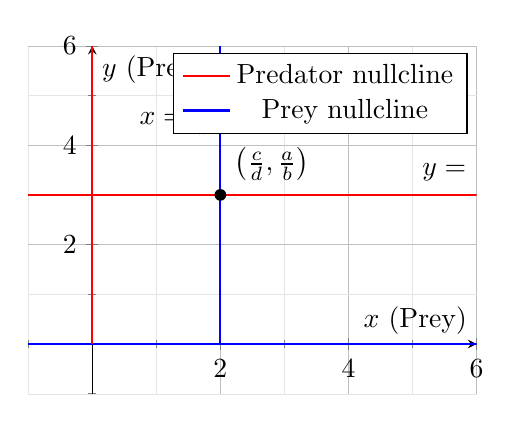
\begin{tikzpicture}
                \begin{axis}[
                    axis lines = middle,
                    view     = {0}{90},
                    xlabel = \( x \) (Prey),
                    ylabel = \( y \) (Predator),
                    ymin = -1, ymax = 6,
                    xmin = -1, xmax = 6,
                    domain=-1:6,
                    samples=200,
                    width=0.6\linewidth,
                    height=6cm,
                    grid=both,
                    minor tick num=1,
                    major grid style={line width=.2pt,draw=gray!50},
                    minor grid style={line width=.1pt,draw=gray!20},
                ]
                % Prey nullcline (horizontal line)
                \addplot[red, thick] {3};
                % trvial nullclines (axes)
                \addplot[blue, thick] {0};
                \node at (axis cs:5,3) [anchor=south west] {\( y = \frac{a}{b} \)};
                % Predator nullcline (vertical line)
                \addplot[red, thick] coordinates {(0,0) (0,6)};
                \addlegendentry{Predator nullcline}
                % trvial nullclines (axes)
                \addplot[blue, thick] coordinates {(2,0) (2,6)};
                \addlegendentry{Prey nullcline}


                \node at (axis cs:2,5) [anchor=north east] {\( x = \frac{c}{d} \)};
                % Fixed point marker
                \node at (axis cs:2,3) [circle,fill,inner sep=1.5pt,label=above right:{\(\left(\frac{c}{d}, \frac{a}{b}\right)\)}] {};
                \end{axis}
            \end{tikzpicture}
            \caption{Nullclines of the Lotka-Volterra model showing the prey nullcline (horizontal line) and predator nullcline (vertical line). The intersection point represents the coexistence equilibrium.}
        \end{figure}
        And a figure for the vector field is shown below:
        \begin{figure}[h!]
            \centering
            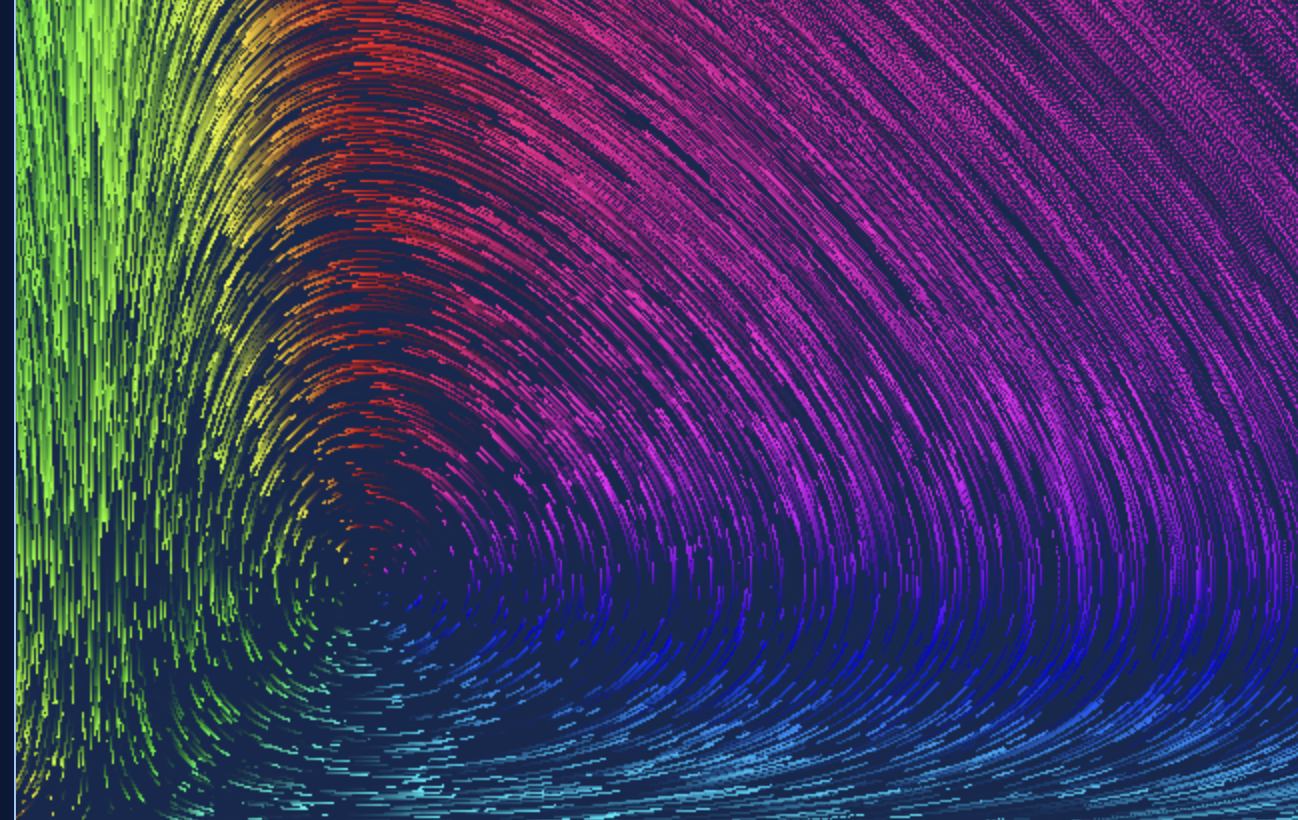
\includegraphics[width=0.6\linewidth]{predprey.png}
            \caption{Vector field of the Lotka-Volterra model showing the circular flow around
            the fixed point \(\left(\frac{c}{d}, \frac{a}{b}\right)\).}
        \end{figure}
\end{example}


\begin{example}[Simple Pendulum]
    Consider a simple pendulum of length \( L \) and mass \( m \) under the influence of gravity \( g \). The angle \( \theta(t) \) that the pendulum makes with the vertical satisfies the second-order ODE:
    $$
    \theta'' + \frac{g}{L} \sin(\theta) = 0
    $$
    To convert this into a system of first-order ODEs, we let:
    $$\begin{cases}
    x := \theta  \quad x' = \theta' = y \\
    y := \theta' \quad y' = \theta'' = -\frac{g}{L} \sin(x)
    \end{cases}$$

    Consider the fixed points of this system by setting \( x' = 0 \) and \( y' = 0 \). Then we have:
    $$(x^*, y^*) = (n\pi, 0) \quad n \in \mathbb{Z}$$
    The case where \( n \) is even (e.g., \( 0, 2, 4, \ldots \)) corresponds to the pendulum hanging straight down (stable equilibrium), while the case where \( n \) is odd (e.g., \( 1, 3, 5, \ldots \)) corresponds to the pendulum being inverted (unstable equilibrium).
    
    Consider the nullclines:
    \begin{itemize}
        \item \( x' = 0 \) (horizontal nullcline): \( y = 0 \)
        \item \( y' = 0 \) (vertical nullcline): \( \sin(x) = 0 \implies x = n\pi, n \in \mathbb{Z} \) And we have, for $y$:
        
    \end{itemize}

    A vector field of the system is shown below:
        \begin{figure}[h!]
            \centering
            
\includegraphics[width=0.6\linewidth]{pendulum.png}
            \caption{Vector field of the simple pendulum system showing the fixed points at \( (n\pi, 0) \).}
        \end{figure}

\end{example}

\paragraph{Systems of ODEs as Matrices}
A system of ODEs can be expressed in matrix form as:
$$\mathbf{x}' = A\mathbf{x} + \mathbf{b}(t)
$$where \( \mathbf{x} \) is the state vector, \( A \) is a matrix of coefficients, and \( \mathbf{b}(t) \) is a vector of functions.

\begin{definition}[General System of ODEs]
    WLOG, for a system of 2 ODEs with $x$ and $y$, we write:
    $$\begin{cases}
    x' = f(t, x, y) \\
    y' = g(t, x, y)
    \end{cases}$$
    where \( f \) and \( g \) are given functions:
    $$
    f(t, x, y) = p_{11}(t)x + p_{12}(t)y + g_1(t) \\
    g(t, x, y) = p_{21}(t)x + p_{22}(t)y + g_2(t)
    $$
    We can express this in matrix form as:
    \begin{equation}
    \begin{bmatrix}x' \\ y'
    \end{bmatrix} = \begin{bmatrix}
    p_{11}(t) & p_{12}(t) \\
    p_{21}(t) & p_{22}(t)
    \end{bmatrix} \begin{bmatrix}x \\ y
    \end{bmatrix} + \begin{bmatrix}g_1(t) \\ g_2(t)
    \end{bmatrix}
    \end{equation}

    Furthermore, we generalize this to \( n \) dimensions, and the inhomogeneous, non-autonomous system of linears ODEs is given by:
    \begin{align*}
    \mathbf{x}'_1 &= \sum^n_{j=1} P_{1j}(t)x_j + g_1(t) \quad i = 1, 2, \ldots, n \\
     & \vdots \\
    \mathbf{x}'_n &= \sum^n_{j=1} P_{nj}(t)x_j + g_n(t)
    \end{align*}
    or in matrix form:
    \begin{equation}
    \mathbf{x}' = A(t)\mathbf{x} + \mathbf{G}(t)
    \end{equation}
    where \( A(t) \) is an \( n \times n \) matrix of functions, \( \mathbf{x} \) is the state vector, and \( \mathbf{G}(t) \) is the inhomogeneous term.
\end{definition}

\begin{theorem}[Existence and Uniqueness for Systems of ODEs]
    If $p_{ij}(t)$ and $g_i(t)$ are continuous on an open interval $I = (a, b)$ containing $t_0$ for all $i, j = 1, 2, \ldots, n$, then the initial value problem
    $$\mathbf{x}' = A(t)\mathbf{x} + \mathbf{G}(t), \quad \mathbf{x}(t_0) = \mathbf{x}_0$$
    has a unique solution on the interval \( I \).
\end{theorem}

\begin{example}[Linear, homogeneous and autonomous]
    Consider the simple ODE system:
    $$
        \textbf{x}' = A\textbf{x} +\textbf{b}
    $$
    We cosidner the fix points by setting \( \textbf{x}' = 0 \):
    $$A\textbf{x} + \textbf{b} = 0 \implies A\textbf{x} = -\textbf{b}$$
    If \( A \) is invertible, then the fixed point is given by:
    $$\textbf{x}^* = -A^{-1}\textbf{b}$$
    If \( A \) is not invertible, then there are either no fixed points or infinitely many fixed points. Now, we let $\textbf{y} = \textbf{x} + A^{-1}\textbf{b}$, then we have:
    $$\textbf{y}' =\textbf{x}'$$
    we have:
    $$Ay = A\textbf{x} + \textbf{b} = \textbf{x}' = \textbf{y}'$$
    Thus, the system reduces to:
    $$\textbf{y}' = A\textbf{y}$$
    which is a linear, homogeneous, and autonomous system. The fixed point of this system is given by:
    $$\textbf{y}^* = 0$$
\end{example}

\begin{example}[Simple ODEs]
    Consider the system of ODEs:
    $$
    \textbf{x}' = \begin{bmatrix} 1 & 0 \\ 0 & -2
    \end{bmatrix}\textbf{x} 
    $$
    and the initial condition:
    $$
    \textbf{x}(0) = \begin{bmatrix} x_0 \\ y_0
    \end{bmatrix}
    $$
    Then we can consider the solutions:
    $$x_1(t) = x_0 e^{t}$$
    $$x_2(t) = y_0 e^{-2t}$$
    or we can write the solution in vector form:
    $$\textbf{x}(t) = x_0 \begin{bmatrix}
        1 \\ 0
    \end{bmatrix} e^{t} + y_0 \begin{bmatrix}
        0 \\ 1
    \end{bmatrix} e^{-2t}
    $$

    The fixed point and nullclines are given by:
    $$\textbf{x}^* = \begin{bmatrix}0 \\ 0
    \end{bmatrix}$$
    The nullclines are given by:
    \begin{itemize}
        \item \( x' = 0 \): \( x = 0 \) (vertical line)
        \item \( y' = 0 \): \( y = 0 \) (horizontal line)
    \end{itemize}
    
    \textbf{Stability of Nullclines} The $x$-nullcline since it goes to the origin as $t \to -\infty$ and away from the origin as $t \to \infty$, while the $y$-nullcline goes to the origin as $t \to \infty$ and away from the origin as $t \to -\infty$. 
        \begin{figure}[h!]
            \centering
            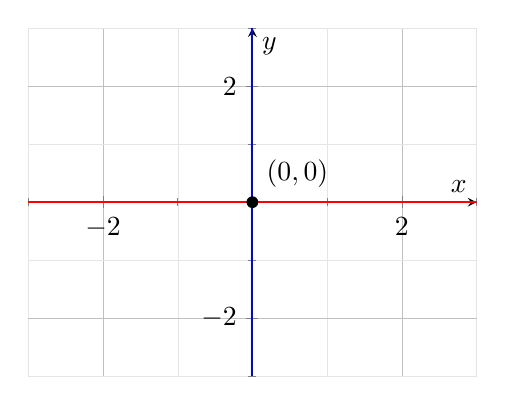
\begin{tikzpicture}
                \begin{axis}[
                    axis lines = middle,
                    view     = {0}{90},
                    xlabel = \( x \),
                    ylabel = \( y \),
                    ymin = -3, ymax = 3,
                    xmin = -3, xmax = 3,
                    domain=-3:3,
                    samples=200,
                    width=0.6\linewidth,
                    height=6cm,
                    grid=both,
                    minor tick num=1,
                    major grid style={line width=.2pt,draw=gray!50},
                    minor grid style={line width=.1pt,draw=gray!20},
                ]
                % x-nullcline (vertical line)
                \addplot[blue, thick] coordinates {(0,-3) (0,3)};
                % y-nullcline (horizontal line)
                \addplot[red, thick] coordinates {(-3,0) (3,0)};
                % Fixed point marker
                \node at (axis cs:0,0) [circle,fill,inner sep=1.5pt,label=above right:{\((0, 0)\)}] {};
                \end{axis}
            \end{tikzpicture}
            \caption{Phase portrait of the simple ODE system showing the nullclines and the fixed point at the origin.}
        \end{figure}
        \textbf{Note - Stability} The stability here really means that the trajectories approach or move away from the fixed point along the nullclines, this does not mean for perturbation along the nullclines.
        \textbf{Saddle Node} The fixed point is a saddle node (since one eigenvalue is positive and the other is negative). The trajectories in the phase plane are shown below:
\end{example}

\begin{example}[Linear Algebra]
    Consider the system of ODEs:
    $$
    \textbf{x}' = A\textbf{x}
    $$
    where \( A \) is a constant matrix. Consider:
    \begin{align*}
        \textbf{x} &= \vec{v} e^{\lambda t} \\
        \textbf{x}' &= \lambda \vec{v} e^{\lambda t} \\
        &= A\vec{v} e^{\lambda t} = A\textbf{x}
    \end{align*}
    Thus, we have:
    
    \begin{equation}
    A\vec{v} = \lambda \vec{v}
        \end{equation}
    which is the eigenvalue problem. 
\end{example}

\begin{example}[Superposition]

    Assume $x_1(t)$ and $x_2(t)$ are solutions to the system of ODEs:
    $$\textbf{x}' = A\textbf{x}$$
    Then, any linear combination of these solutions is also a solution:
    $$\textbf{x}(t) = c_1 x_1(t) + c_2 x_2(t)$$
    where \( c_1 \) and \( c_2 \) are constants. This is due to the linearity of the system.
\end{example}

\begin{definition}[General Eigenproblem for n-dim ODEs System]
    Combining the above ideas, consider the system:
    $$\textbf{x}' = A\textbf{x}$$
    where \( A \in \mathbb{R}^{n \times n} \). We define the \textit{specturm} as:
    \begin{equation}
    \sigma(A) = \{(\lambda_i, \vec{v}_i) \in \mathbb{C} \times \mathbb{C}^n : A\vec{v}_i = \lambda_i \vec{v}_i, i = 1, 2, \ldots, n\}
    \end{equation}
    where \( \lambda_i \) are the eigenvalues and \( \vec{v}_i \) are the corresponding eigenvectors. The general solution to the system can be expressed as:
    \begin{equation}
            \textbf{x}(t) = \sum_{i=1}^{n} c_i \vec{v}_i e^{\lambda_i t}
    \end{equation}
    where \( c_i \) are constants determined by the initial conditions.
\end{definition}

\begin{example}
    Consider the following system of ODEs:
    $$
    \textbf{x}' = \begin{bmatrix} 0 & 1 \\ 1 & 0
    \end{bmatrix}\textbf{x}
    $$
    We find the eigenvalues and eigenvectors by solving the characteristic polynomial:
    \begin{align*}
    \det(A - \lambda I) &= \det\begin{bmatrix} -\lambda & 1 \\ 1 & -\lambda
    \end{bmatrix} \\
    &= \lambda^2 - 1 = 0 \\
    \implies \lambda_1 &= 1, \quad \lambda_2 = -1
    \end{align*}
    The corresponding eigenvectors are:
    \begin{align*}
    \vec{v}_1 &= \begin{bmatrix} 1 \\ 1
    \end{bmatrix}, \quad \vec{v}_2 = \begin{bmatrix} -1 \\ 1
    \end{bmatrix}
    \end{align*}
    Thus, the general solution to the system is:
    $$\textbf{x}(t) = c_1 \begin{bmatrix} 1 \\ 1
    \end{bmatrix} e^{t} + c_2 \begin{bmatrix} -1 \\ 1
    \end{bmatrix} e^{-t}$$
    where \( c_1 \) and \( c_2 \) are constants determined by the initial conditions.

    Consider the phase portait. If we start on the span of $ [-1, 1]^T$, then we go to the origin as $t \to \infty$. If we start on the span of $ [1, 1]^T$, then we go away from the origin as $t \to \infty$. Then, the trivial fixed point is a saddle node.
\end{example}

\begin{definition}[Computing Eigenvalues via Trace and Determinant]
    Consider matrix $A \in \mathbb{R}^{2 \times 2}$. We compute the eigenvalues by solving the characteristic polynomial:
    \begin{align*}
    0 &= \det(A - \lambda I) \\
    &= \lambda^2 - \text{tr}(A)\lambda + \det(A) \\
    \implies \lambda_{1,2} &= \frac{\text{tr}(A) \pm \sqrt{\text{tr}(A)^2 - 4\det(A)}}{2}
    \end{align*}

    If the roots are real, there are four cases that coud emerge from this (WLOG): 
    \begin{itemize}
        \item $\lambda_1 > \lambda_2 > 0$: We see much faster growth in the span assocaited with $\lambda_1$.
        \item $\lambda_1 < \lambda_2 < 0$: We see much faster decay in the span assocaited with $\lambda_1$.
        \item $\lambda_1 < 0 < \lambda_2$: We would see the span assocaited with $\lambda_2$ dominate as $t \to \infty$ and the span assocaited with $\lambda_1$ dominate as $t \to -\infty$. This is a saddle node.
        \item $\lambda_2  = 0 < \lambda_1$: Along the span of $v_2$, we would see horizontal line, as we growth only along the span of $v_1$. 
        \item $\lambda_1 = \lambda_2 > 0$: Along the span of $v_2$, we would see horizontal line, as we decay only along the span of $v_1$.
        \item $\lambda_1 = \lambda_2 = 0$: The system is trivial, and all points are fixed points.
        \item $\lambda_1 = \lambda_2 < 0$: It is a inward star that everything goes to the origin.
        \item $\lambda_1 = \lambda_2 > 0$: It is an outward star that everything goes away from the origin.
    \end{itemize}
\end{definition}

\begin{definition}[Complex Eigenvalues]
    Consider the case where the eigenvalues are complex, i.e., \( \lambda = \alpha \pm i\beta \) with \( \beta \neq 0 \). The general solution to the system can be expressed as:
    $$\textbf{x}(t) = e^{\alpha t} \left( c_1 \text{Re}(\vec{v} e^{i\beta t}) + c_2 \text{Im}(\vec{v} e^{i\beta t}) \right)$$
    where \( \vec{v} \) is the complex eigenvector corresponding to \( \lambda \), and \( c_1, c_2 \) are constants determined by the initial conditions.

    This would lead to the following definition of a radial and angular component:
    \begin{equation}
    v(t) = ve^{\alpha t} \mathrm{cis} (\beta t)
    \end{equation}
    where \( r(t) \) represents the radial distance from the origin and \( \theta(t) \) represents the angular position. So, for a general solution, we have:
    \begin{equation}
    \textbf{x}(t) = \sum_i c_i v_i e^{\alpha_i t} \mathrm{cis} (\beta_i t)
    \end{equation}
    The behavior of the system depends on the sign of \( \alpha \) and $\beta$:
    \begin{itemize}
        \item If \( \alpha > 0 \) the system spirals outward (complex source).
        \begin{itemize}
            \item If \( \beta > 0 \), the systems sprial counter-clockwise.
            \item If \( \beta < 0 \), the systems sprial clockwise.
        \end{itemize}
        \item If \( \alpha < 0 \) the system spirals inward (complex sink).
        \begin{itemize}
            \item If \( \beta > 0 \), the systems sprial counter-clockwise.
            \item If \( \beta < 0 \), the systems sprial clockwise.
        \end{itemize}
        \item If \( \alpha = 0 \) the system is a center (closed orbits).
        \begin{itemize}
            \item If \( \beta > 0 \), the systems sprial counter-clockwise.
            \item If \( \beta < 0 \), the systems sprial clockwise.       
        \end{itemize}
    \end{itemize}
\end{definition}

\paragraph{Complex Eigenvalues Resolves to Real Numbers} Consider eigenvalues $\lambda = \alpha \pm i\beta \in \mathbb{C}$ with $v = \textbf{p} + i\textbf{q}\in \mathbb{C}^n$. Then, the general solution $x: \mathbb{R} \to \mathbb{R}^n$ is given by:
\begin{equation}
\textbf{x}(t) = c_1 e^{\lambda t} \textbf{v} + c_2 e^{\bar{\lambda} t} \bar{\textbf{v}}
\end{equation}
where $c_1, c_2 \in \mathbb{C}$.

We also have:
$$
    \bar{\textbf{x}} = \bar{c_1} e^{\bar{\lambda} t} \bar{\textbf{v}} + \bar{c_2} e^{\lambda t} \textbf{v}
$$
So, we can say that:
$$
c_1 = \bar{c_2}, \quad c_2 = \bar{c_1}
$$
Let $c_1 =  \delta + i\gamma$, then $c_2 = \delta - i\gamma$. Thus, we have:
\begin{equation}
\textbf{x}(t) = (\delta + i\gamma)e^{(\alpha + i\beta)t}(\textbf{p} + i\textbf{q}) + (\delta - i\gamma)e^{(\alpha - i\beta)t}(\textbf{p} - i\textbf{q}) \\
\end{equation}
Seperating the real and imaginary parts, we have:
\begin{equation}
\textbf{x}(t) = \delta (ve^{\lambda t} + \bar{v}e^{\bar{\lambda} t}) + i\gamma (ve^{\lambda t} - \bar{v}e^{\bar{\lambda} t})
\end{equation}
By the Euler's formula, we have:
\begin{equation}
\textbf{x}(t) = 2\delta \mathrm{Re}(ve^{\lambda t}) - 2\gamma \mathrm{Im}(ve^{\lambda t}) \in \mathbb{R}^n
\end{equation}

\paragraph{Generalized eigenvectors and solution for a defective matrix}
Consider the matrix
\[
A=\begin{bmatrix}2 & 1\\[4pt]0 & 2\end{bmatrix},
\]
which has a double eigenvalue \(\lambda=2\) but only one linearly independent eigenvector
\[
v=\begin{bmatrix}1\\[4pt]0\end{bmatrix}.
\]

To complete a Jordan chain of length two we seek a generalized eigenvector \(v_g\) satisfying
\begin{equation}
(A-\lambda I)\,v_g = v. \label{eq:gen-eig}
\end{equation}
For this \(A\) we have \(A-2I=\begin{bmatrix}0&1\\0&0\end{bmatrix}\). Choosing the convenient solution
\[
v_g=\begin{bmatrix}0\\[4pt]1\end{bmatrix}
\]
indeed yields \((A-2I)v_g=v\), so \eqref{eq:gen-eig} holds.

The two linearly independent solutions corresponding to this Jordan chain are
\begin{equation}
x_1(t)=v\,e^{\lambda t} = \begin{bmatrix}1\\[4pt]0\end{bmatrix} e^{2t}, \label{eq:sol1}
\end{equation}
and
\begin{equation}
x_2(t)=(v_g + t\,v)\,e^{\lambda t} = \left(\begin{bmatrix}0\\[4pt]1\end{bmatrix} + t\begin{bmatrix}1\\[4pt]0\end{bmatrix}\right)e^{2t}. \label{eq:sol2}
\end{equation}
One checks directly that these satisfy \(x_i'(t)=Ax_i(t)\) using \(Av=\lambda v\) and \(Av_g=\lambda v_g + v\).

Therefore the general solution of \(\mathbf{x}'=A\mathbf{x}\) is the linear combination
\begin{equation}
\mathbf{x}(t)=C_1\,x_1(t) + C_2\,x_2(t)
= e^{\lambda t} \begin{bmatrix}
C_1 + C_2 t \\[4pt] C_2
\end{bmatrix}
\end{equation}
The phase portrait of this system is shown below:
% insert later

\begin{definition}[Trace-Determinant Plane]
    We found that we can find the eigenvalues of a \( 2 \times 2 \) matrix \( A \) using:
    $$
    \lambda_{1,2} = \frac{\text{tr}(A) \pm \sqrt{\text{tr}(A)^2 - 4\det(A)}}{2}
    $$
    where
    \begin{itemize}
        \item \( \text{tr}(A) = \lambda_1 + \lambda_2 = a_{11} + a_{22} \) is the trace of \( A \)
        \item \( \det(A) = \lambda_1 \lambda_2 = a_{11}a_{22} - a_{12}a_{21} \) is the determinant of \( A \)   
    \end{itemize}
    And we have the following analysis:
    \begin{itemize}
        \item If \( \det(A) < 0 \) and \( \text{tr}(A) > 0 \), then \( \lambda_1 > 0 > \lambda_2 \) (saddle node).
        \item Consider the discriminant boundry \( \text{tr}(A)^2 - 4\det(A) = 0 \), it is a parabola that upward opening with vertex at the origin. Consider region above that, where there is complex eigenvalues:
        \begin{itemize}
            \item If \( \text{tr}(A) > 0 \) and \( \det(A) > 0 \), then \( \alpha = \text{tr}(A)/2 > 0 \) (spiral source).
            \item If \( \text{tr}(A) < 0 \) and \( \det(A) > 0 \), then \( \alpha = \text{tr}(A)/2 < 0 \) (spiral sink).
            \item If \( \text{tr}(A) = 0 \) and \( \det(A) > 0 \), then \( \lambda_1 = -\lambda_2 = i\beta \) (center).
        \end{itemize}
        \item Consider the region below the discriminant boundry, where there is real eigenvalues:
        \begin{itemize}
            \item If \( \text{tr}(A) > 0 \) and \( \det(A) > 0 \), then \( \lambda_1 \geq \lambda_2 > 0 \) (nodal source).
            \item If \( \text{tr}(A) < 0 \) and \( \det(A) > 0 \), then \( 0 > \lambda_1 \geq \lambda_2 \) (nodal sink).
        \end{itemize}
        \item \textbf{Degenerate Star Node} Consider the line \( \text{tr}(A)^2 - 4\det(A) = 0 \).
        \item \textbf{Lines of Nodes} Consider the line \( \det(A) = 0 \).
    \end{itemize}
\end{definition}

\subsection{Wronskian and Fundamental Matrix}
\begin{definition}[Functionals]
    A functional is a mapping from a vector space of functions to the real numbers. For example, consider the space of continuous functions on an interval \( [a, b] \), denoted by \( C[a, b] \). A functional \( J: C[a, b] \to \mathbb{R} \) could be defined as:
    $$
    J[f] = \int_a^b f(x) \, dx
    $$
    for any function \( f \in C[a, b] \).
\end{definition}

\paragraph{Motivation} For an $n$th-order differential equation we need $n$ linearly independent solutions to form the general solution. These solutions constitute a basis of the solution space, so we must check whether a given set of solutions is linearly independent.

\begin{definition}[Wronskian]
    Consider \( n \) functions \( x_1(t), x_2(t), \ldots, x_n(t) \) for which \( x: \mathbb{R} \to \mathbb{R}^n \) that are solutions of a $n$th-order linear differential equation on an interval \( I \). The Wronskian \( W(t) \) is defined as the determinant of the matrix whose columns are formed by the functions and their derivatives up to order \( n-1 \):
    \begin{equation}
    W(t) = \det\begin{bmatrix}
    x_1(t) & x_2(t) & \cdots & x_n(t) \\
    x_1'(t) & x_2'(t) & \cdots & x_n'(t) \\
    \vdots & \vdots & \ddots & \vdots \\
    x_1^{(n-1)}(t) & x_2^{(n-1)}(t) & \cdots & x_n^{(n-1)}(t)
    \end{bmatrix} 
    \end{equation}
    Iff there exist \( t \) in interval \( I \) such that \( W(t) \neq 0 \), then the functions \( x_1(t), x_2(t), \ldots, x_n(t) \) are linearly independent on \( I \).

\end{definition}

\begin{example}
    Let $f(x) = \cos (mx)$ and $g(x) = \sin (mx)$ for some constant $m \neq 0$. We compute the Wronskian:
    \begin{align*}
    W(f, g)(x) &= \det\begin{bmatrix}
    \cos(mx) & \sin(mx) \\
    -m\sin(mx) & m\cos(mx)
    \end{bmatrix} \\
    &= m\cos^2(mx) + m\sin^2(mx) \\
    &= m(\cos^2(mx) + \sin^2(mx)) \\
    &= m \neq 0
    \end{align*}
    Since \( W(f, g)(x) \neq 0 \) for all \( x \), the functions \( \cos(mx) \) and \( \sin(mx) \) are linearly independent on \( \mathbb{R} \).
\end{example}
\paragraph{Trading order for dimension} Consider the $n$th-order ODE:
$$a_n(t)x^{(n)} + a_{n-1}(t)x^{(n-1)} + \ldots + a_1(t)x' + a_0(t)x = g(t)$$
where \( a_n(t) \neq 0 \) on an interval \( I \). We can convert this into a system of first-order ODEs by defining:
$$\begin{cases}
x_1 = x \\
x_2 = x' \\
x_3 = x'' \\
\vdots \\
x_n = x^{(n-1)}
\end{cases}$$
Then, we have solution $x: \mathbb{R} \to \mathbb{R}^n$ given by:
$$
x = v_1 e^{\lambda_1 t} + v_2 e^{\lambda_2 t} + \ldots + v_n e^{\lambda_n t}
$$
where \( v_i \) are the eigenvectors and \( \lambda_i \) are the eigenvalues of the corresponding matrix \( A \). Then, we can define the Wronskian for this system as:
\begin{equation}
W(v_1e^{\lambda_1 t}, v_2 e^{\lambda_2 t}, \ldots, v_n e^{\lambda_n t}) = 
\begin{vmatrix}
v_1 e^{\lambda_1 t} & v_2 e^{\lambda_2 t} & \ldots & v_n e^{\lambda_n t} 
\end{vmatrix} = e^{(\lambda_1 + \lambda_2 + \ldots + \lambda_n)t} \begin{vmatrix}
v_1 & v_2 & \ldots & v_n 
\end{vmatrix}
\end{equation}
Which the first term is never zero, so the Wronskian is non-zero iff the eigenvectors are linearly independent. The basis $\{v_1 e^{\lambda_1 t}, v_2 e^{\lambda_2 t}, \ldots, v_n e^{\lambda_n t}\}$ is a fundamental called the fundamental set of solutions.

\paragraph{General Planer Systems} Consider the system of ODEs:
$$\textbf{x}' = A\textbf{x}$$
where \( A \in \mathbb{R}^{2 \times 2} \).
We define the fundamental matrix \( \Phi(t) \) as:
\begin{equation}
\Phi(t) = \begin{bmatrix}
x_1(t) & x_2(t) \\ 
y_1(t) & y_2(t)
\end{bmatrix}
\end{equation}
where \( (x_1(t), y_1(t)) \) and \( (x_2(t), y_2(t)) \) are two linearly independent solutions of the system. The Wronskian of the system is given by:
\begin{equation}
W(t) = \det(\Phi(t)) = x_1(t)y_2(t) - x_2(t)y_1(t)
\end{equation}
The Wronskian satisfies the differential equation:
\begin{equation}
W'(t) = \text{tr}(A) W(t)
\end{equation}
with the solution:
\begin{equation}
W(t) = W(0) e^{\text{tr}(A)t}
\end{equation}
where \( W(0) \) is the Wronskian at \( t = 0 \).

\subsection{Stability of Nonlinear Systems in Local Linear Approximation}
\begin{definition}[Change of Variables]
    The change of variable in a higher dimensions, the change of variables related by the Jacobian matrix. WLOG, consider change of variables $F: \mathbb{R}^2 \to \mathbb{R}^2$ and system $x' = Ax$. Let:
    $$
    F(x,y) = \begin{bmatrix}f_1(x,y) \\ f_2(x,y)
    \end{bmatrix}
    $$

    Then, the Jacobian matrix \( J_F \) is given by:
    \begin{equation}
    J_F = \begin{bmatrix}
    \frac{\partial f_1}{\partial x} & \frac{\partial f_1}{\partial y} \\
    \frac{\partial f_2}{\partial x} & \frac{\partial f_2}{\partial y}
    \end{bmatrix}
    \end{equation}
    The change of variables transforms the system \( x' = Ax \) into a new system \( u' = Bu \) where:
    \begin{equation}
    B = J_F A J_F^{-1}
    \end{equation}
    provided that \( J_F \) is invertible.
\end{definition}

\begin{shaded}
\subsubsection*{A reference for simple linear stability analysis.}

\paragraph{Linear Stablity Analysis} Consider the simple linear one-dimensional ODE:
$$y' = f(y)$$
where \( f(y) \) is a differentiable function. Let \( y^* \) be a fixed point, i.e., \( f(y^*) = 0 \). We can perform a linear stability analysis by considering a small perturbation \( \eta(t) = y(t) - y^* \). Then, we have:
\begin{align*}
\eta' &= y' - (y^*)' \\
&= f(y) - 0 \\
&= f(y^* + \eta) \\
&\approx f(y^*) + f'(y^*)\eta \\
&= f'(y^*)\eta = A\eta
\end{align*}
So, we have the linearized system:
$$\eta' = A\eta$$
where \( A = f'(y^*) \). The stability of the fixed point \( y^* \) is determined by the sign of \( A \).
\end{shaded}

\begin{definition}[Linear Stability Analysis in Higher Dimensions]
Consider the two-dimensional system:
$$\begin{cases}
x' = f(x, y) \\
y' = g(x, y)
\end{cases}$$
where \( f(x, y) \) and \( g(x, y) \) are differentiable functions. Let \( (x^*, y^*) \) be a fixed point. We let perturbations \( u(t) = x(t) - x^* \) and \( v(t) = y(t) - y^* \). Then, we have:
$$
\begin{cases}
    u' &= x' = \cancel{f(x,y)} + \frac{\partial f}{\partial x}(x^*, y^*)u + \frac{\partial f}{\partial y}(x^*, y^*)v + \cancel{O(u^2, v^2, uv)} \\
    v' &= y' = \cancel{g(x,y)} + \frac{\partial g}{\partial x}(x^*, y^*)u + \frac{\partial g}{\partial y}(x^*, y^*)v + \cancel{O(u^2, v^2, uv)}
\end{cases}
$$
So we can write the linearized system as:
$$\begin{bmatrix}
u' \\ v'
\end{bmatrix} = J \begin{bmatrix}
u \\ v
\end{bmatrix}$$
where \( J \) is the Jacobian matrix evaluated at the fixed point \( (x^*, y^*) \). This describes the local behavior of the system near the fixed point. Then the stability and behavior is determined by the determinant and trace of the Jacobian matrix \( J \), and hence the eigenvalues and eigenvectors of \( J \).
\end{definition}

\begin{definition}
    Consider the nonlinear pendulum equation:
    $$\theta'' + \frac{g}{L}\sin(\theta) = 0$$
    where \( \theta \) is the angle of the pendulum, \( g \) is the acceleration due to gravity, and \( L \) is the length of the pendulum. We can rewrite this as a system of first-order ODEs by defining:
    $$\begin{cases}
    x_1 = \theta \\
    x_2 = \theta'
    \end{cases}$$
    Then, we have:
    $$\begin{cases}
    x_1' = x_2 \\
    x_2' = -\frac{g}{L}\sin(x_1)    
    \end{cases}$$
    Now, consider the Jacaobian matrix:
    $$J = \begin{bmatrix}
    0 & 1 \\
    -\frac{g}{L}\cos(x_1) & 0
    \end{bmatrix}$$
    
    Consider the fixed point $(n \pi, 0)$ for \( n \in \mathbb{Z} \). We have:
    $$J = \begin{bmatrix}
    0 & 1 \\
    -\frac{g}{L}\cos(n \pi) & 0
    \end{bmatrix} = \begin{bmatrix}
    0 & 1 \\
    -\frac{g}{L}(-1)^n & 0
    \end{bmatrix}$$
    So the derminant is:
    $$\det(J) = -\frac{g}{L}(-1)^n$$
    and the trace is:
    $$\text{tr}(J) = 0$$
    When $n$ is even, we have a positive determinant, so the fixed point is a center. When $n$ is odd, we have a negative determinant, so the fixed point is a saddle node.
\end{definition}

\end{document}